% Annals of Applied Statistics submission (IMS imsart class).
% imsart.cls / imsart.sty / spr-ims-nameyear.bst are included (VTeX texsupport.ims-aoas,
% MIT licence, see LICENSE-imsart);
% the IMS class is used. Otherwise the document falls back to the article class
% with minimal stand-ins for the imsart front-matter macros, so it always compiles.
\IfFileExists{imsart.cls}{%
  \documentclass[aoas,preprint]{imsart}\def\IMSfallback{0}%
}{%
  \documentclass[11pt]{article}\def\IMSfallback{1}%
}

\makeatletter
\ifnum\IMSfallback=1
  \usepackage[margin=1in]{geometry}
  \newcommand{\startlocaldefs}{}
  %\newcommand{\endlocaldefs}{}
  \newenvironment{frontmatter}{}{}
  \newcommand{\runtitle}[1]{}
  \def\IMS@authors{}
  \renewcommand{\author}[2][]{%
    \ifx\IMS@authors\@empty\g@addto@macro\IMS@authors{#2}%
    \else\g@addto@macro\IMS@authors{\and #2}\fi
    \gdef\@author{\IMS@authors}}
  \newcommand{\fnms}[1]{#1}
  \newcommand{\snm}[1]{#1}
  \newcommand{\ead}[2][]{}
  \newcommand{\printead}[2][]{}
  \newcommand{\address}[2][]{}
  % the aug block ends the title block: typeset the title after it
  \newenvironment{aug}{\let\and\relax}{\aftergroup\maketitle}
  \newenvironment{keyword}{\par\noindent\textbf{Keywords:} \ignorespaces}{\par}
  \newcommand{\kwd}[1]{#1;\ }
  \newenvironment{funding}{\section*{Funding}}{}
  \newenvironment{acks}[1][Acknowledgments]{\section*{#1}}{}
  \newenvironment{supplement}{\section*{Supplementary material}}{}
  \newcommand{\stitle}[1]{\textbf{#1.}\ }
  \newcommand{\sdescription}[1]{#1}
\fi
\makeatother

\RequirePackage{amsthm,amsmath,amsfonts,amssymb}
\RequirePackage[authoryear]{natbib}
\RequirePackage[colorlinks,citecolor=blue,urlcolor=blue]{hyperref}
\RequirePackage{graphicx}
\RequirePackage{booktabs}
\RequirePackage{multirow}
\RequirePackage{bm}
\RequirePackage{xcolor}
\makeatletter
% Labels of the other document (main <-> supplement), read from a file of its \newlabel
% lines (made by build.sh); the IMS class does not allow the xr package.
\def\extlabels@nl#1#2{\@ifundefined{r@#1}{\global\@namedef{r@#1}{#2}}{}}
\def\extlabels#1{\IfFileExists{#1}{\begingroup\let\newlabel\extlabels@nl
  \input{#1}\endgroup}{}}
\makeatother
\AtBeginDocument{\extlabels{main-labels.tex}}

\startlocaldefs
\numberwithin{equation}{section}
\theoremstyle{plain}
\newtheorem{proposition}{Proposition}
\theoremstyle{definition}
\newtheorem{remark}{Remark}
% notation
\newcommand{\bx}{\bm{x}}
\newcommand{\bz}{\bm{z}}
\newcommand{\bw}{\bm{w}}
\newcommand{\bv}{\bm{v}}
\newcommand{\bu}{\bm{u}}
\newcommand{\bA}{\bm{A}}
\newcommand{\bQ}{\bm{Q}}
\newcommand{\bH}{\bm{H}}
\newcommand{\bC}{\bm{C}}
\newcommand{\bG}{\bm{G}}
\newcommand{\bK}{\bm{K}}
\newcommand{\btheta}{\bm{\theta}}
\newcommand{\bbeta}{\bm{\beta}}
\newcommand{\bgamma}{\bm{\gamma}}
\newcommand{\bmeta}{\bm{\eta}}
\newcommand{\logit}{\operatorname{logit}}
\newcommand{\expit}{\operatorname{expit}}
\newcommand{\E}{\mathbb{E}}
\newcommand{\Var}{\operatorname{Var}}
\newcommand{\Normal}{\mathcal{N}}
\newcommand{\sphere}{\mathbb{S}^2}
\newcommand{\todo}[1]{\textcolor{red}{[TODO: #1]}}
\providecommand{\bseriesno}[1]{#1}% used by spr-ims-nameyear.bst for series volumes
%\endlocaldefs

\setcounter{secnumdepth}{2}
\renewcommand{\thetable}{S\arabic{table}}
\renewcommand{\thefigure}{S\arabic{figure}}
\renewcommand{\thesection}{S\arabic{section}}
\begin{document}

\begin{frontmatter}
\title{Supplementary Material for ``Escalation or shared episodes? A joint
spatio-temporal model of armed conflict and social unrest''}
\runtitle{Supplementary Material}
\begin{aug}
\author[A]{\fnms{Stefano}~\snm{Castruccio}\ead[label=e1]{scastruc@nd.edu}}
\author[B]{\fnms{Richard}~\snm{Marcantonio}}
\address[A]{Department of Applied and Computational Mathematics and Statistics,
University of Notre Dame\printead[presep={,\ }]{e1}}
\address[B]{Kroc Institute for International Peace Studies, Keough School of
Global Affairs, University of Notre Dame}
\end{aug}
\end{frontmatter}

This supplement contains the detailed tables and figures referred to in the main paper.
Equation, section and table numbers without the prefix S refer to the main paper.

\section{Data}\label{supp:data}

\subsection{Construction of the cell-week table}\label{supp:data-table}

The grid consists of all $0.5^\circ$ cells that intersect a country polygon of
Natural Earth (1:10m), excluding cells without a terrestrial biome (rock and ice, and
large lakes). Each cell is assigned to the country that contains its centroid. A
coastal cell whose centroid falls in the sea is assigned to the nearest country. Every
cell-week appears exactly once, and national indicators are attached through the
assigned country, with the exceptions described below. The result is 59{,}339 cells observed for up to 366 weeks.

The table built by the original pipeline differs in one important respect.
About 8.5\% of its 34.7 million distinct cell-weeks (before the biome exclusion)
occur more than once, with multiplicities such as $2^k$, $3^k$ and $2\cdot 3^k$, the
signature of many-to-many joins between the grid and polygons of countries, IPC
regions and national indicators. These copies make up 50.5\% of its 70.0 million
rows. The copies of a cell-week share its events but often disagree on the
covariates. Among duplicated cell-weeks, the copies differ in the EPI and the
liberal democracy index in 62\% of cases, in GDP in 49\%, in the IPC phases in about
25\% and in the climate variables in 7--11\%. We do not know why the climate values
of a cell differ between copies; the original pipeline does not record which
polygon each copy comes from. We keep the whole first row of each cell-week, so that
all covariates of a row come from the same copy. The climate values of duplicated
cell-weeks are therefore those of an arbitrary copy, and this part of the error is
retained rather than repaired. The climate covariates are controls in the joint
models and the conclusions do not rest on their coefficients. IPC
phase populations are the exception: they are averaged over the copies. Five national
indicators (EPI, liberal democracy index, greenhouse gas emissions, material and
ecological footprint) are re-attached for each country and year from the cells of
that country that were not duplicated. When a country-year has no value in these
cells, which happens when the indicator is missing for that country, the code falls
back to the most common value of the kept first copies of that country-year. Since
every country has non-duplicated cells, such values come from copies joined to a
neighbouring country's polygon. The fallback therefore can give a country its
neighbour's value and turns a missing value into an observed one, so the missingness
indicator is not set. In the whole repaired table, 14.5\% of rows take at least one
national indicator from this fallback. Access to electricity is not re-attached at
all: every cell-week keeps the value of its first copy, which in cells that had copies
can come from a neighbouring country. It is therefore not constant within a
country-year, and its decomposition into between- and within-country parts mixes differences across borders with change
over time. GDP per capita is a national quantity: World Bank GDP of the country
divided by the sum of the GHSL population of its cells, and it is constant within
each country-year. Section~\ref{sec:app-data} describes the consequences of the
duplication for the original analysis.

Two features of ACLED matter for modelling. First, geographic coverage expanded over
time, and several countries entered the dataset after 2018. Cell-weeks in a country
before its coverage start are \emph{unobserved}, not event free, so they are removed
rather than coded as zeros. Coverage start dates are taken from ACLED's country
coverage table. Territories not listed there take the date of the country or region
that contains them. Before the biome exclusion, coverage removes 7{,}078{,}822
cell-weeks in 79 countries and territories; 3{,}998{,}319 of them are in Antarctica,
which the biome exclusion would remove in any case. The event history is treated as
incomplete in the first four covered weeks. After both exclusions the table has
19{,}364{,}639 cell-weeks.
Second, the probability that an event is recorded depends on media and partner
density, so the outcome combines occurrence and reporting
\citep{weidmann2016closer}. The two are not separately identified
without auxiliary information. The latent fields of Section~\ref{sec:methods}
absorb spatially smooth reporting differences together with unmeasured drivers of
risk, and we interpret them accordingly. Reporting intensity also changes over time
and by country, for example when ACLED adds sources or partners. The year effects are
global, and at test time they are held at their 2022 value, so they cannot absorb
country-specific changes in reporting. Such changes may explain part of the rise in
recorded unrest above, and they can inflate both the estimated state dependence and
the persistence of the space-time fields.

ACLED also codes the spatial and temporal precision of each event. An event whose
exact location is unknown is placed at the centroid of the town or administrative
unit named in the source, and an event whose exact date is unknown at a nominal date
within the reported period. The data available to us are weekly counts by cell, and
they carry no precision codes, so we cannot filter or weight events by precision.
Imprecisely located events accumulate in the cells that contain administrative
centroids and capitals. This can inflate both the persistence of events in those
cells and the cell-level latent effects estimated there, and it is one more reason
to read those effects as recorded rather than actual risk.

\subsection{Covariates and missing values}\label{supp:data-cov}

The climate variables enter all models only through their means over the four weeks
before the current week, so that they precede the outcome; values of the current
week are not used. The original analysis also used the current week's values. A raw temperature
means different things in different climates. In the latent models, the five
climate variables (maximum and minimum temperature, precipitation, drought and
PM$_{2.5}$) therefore enter as standardised anomalies with respect to a cell- and
calendar-month-specific climatology estimated from the training years 2018--2022,
\[
z_{st} = \bigl(x_{st} - \bar{x}_{s,\mathrm{m}(t)}\bigr) / \mathrm{sd}_{s,\mathrm{m}(t)},
\]
where $\mathrm{m}(t)$ is the calendar month of week $t$. Precipitation is
transformed to $\log(1 + x)$ before the anomaly is computed. In dry seasons of arid
cells the training-period standard deviation can be zero or close to zero, and any
later rain would then give an extreme anomaly. We therefore floor
$\mathrm{sd}_{s,\mathrm{m}}$ at the 10th percentile of the positive cell-month
standard deviations of the same variable, and set $z_{st} = 0$ where the
climatological standard deviation is zero. In the AME region the floor applies, by
construction, to 10\% of the 164{,}628 cell-months for temperature and precipitation.
The drought index is constant over the training years in 138{,}600 cell-months (84\%),
so its anomaly is zero there, and the floor applies to a further 1.3\%. The drought
anomaly is therefore informative only in a minority of cell-months. The PM$_{2.5}$
anomaly is worse. Its climatological standard deviation is undefined in 91{,}392
cell-months (56\%), where PM$_{2.5}$ is missing, and the floor computed from the other
cell-months is about $10^{-9}$, so it does not prevent extreme anomalies. The
PM$_{2.5}$ anomaly is missing in 55.5\% of training rows, is then set to zero and has
no missingness indicator. We do not interpret its coefficient. The anomaly coefficients are identified
from variation over time within cells. They are therefore not confounded by the
time-invariant spatial pattern of the climatology. They can still be confounded by
regional shocks that vary over time, since the year effects are global. The cell's
mean over the training years enters separately as a cell-level covariate. A
five-year climatology is noisy, especially for precipitation, and a longer reference
period would be preferable where available. The anomalies are therefore best read
as departures from recent conditions.

\paragraph{Missing covariates.} Table~\ref{tab:covariates} hides substantial
missingness. In the repaired table over the AME region
(4{,}976{,}634 cell-weeks), the IPC phase populations are missing in 62.7\% of rows,
PM$_{2.5}$ in 55.5\%, and GDP in 3.6\%, mainly in South Sudan, Yemen,
Somaliland, Eritrea, Western Sahara and Syria. The other national indicators (EPI,
liberal democracy index, greenhouse gas emissions, material and ecological footprint)
are missing in 0.3\% of rows, at most about 850 cell-weeks in any country. These
shares are after the fallback described in Section~\ref{sec:data-acled}, which fills
some missing values with a neighbouring country's value. The
climate means over the previous four weeks are missing in 1.1\% of rows, and the event
histories in 1.1\%. Over all cell-weeks worldwide the IPC phases
are missing in 89.6\% of rows and precipitation in 20.8\%. IPC analyses are carried
out mainly where food crises are expected, and several of the countries without GDP
data are among the most conflict-affected in the region. Missingness is
therefore unlikely to be at random with respect to the outcome.

Apart from that fallback, we keep missing values as missing through the construction
of the features. In particular, a cell-week without an IPC analysis has a missing IPC value, not a
food-insecure population of zero. All covariates of the latent models other than the
event histories are standardised with training-period means and standard
deviations. Missing values are then set to zero, the training mean, and a
missingness indicator enters the model for each covariate group: one for each
national indicator and one for IPC (Section~\ref{sec:methods-model}).

\begin{table}
\caption{Covariates, resolution and source.}\label{tab:covariates}
\centering\small
\begin{tabular}{@{}lll@{}}
\toprule
Covariate & Resolution & Source \\
\midrule
Minimum / maximum temperature & cell--week & CHIRTS \\
Heat index, wet-bulb globe temperature & cell--week & CHIRTS \\
Precipitation & cell--week & CHIRPS \\
PM$_{2.5}$ & cell--week & CAMS \\
Drought index & cell--week & Global Drought Observatory \\
Events of each type in previous 4 weeks & cell--week & ACLED \\
Population & cell & GHSL \\
River length, lake area & cell & Natural Earth \\
Malaria risk & cell & Malaria Atlas Project \\
Biome & cell & RESOLVE Ecoregions \\
Food insecurity (IPC phases 1--5) & subnational--period & IPC \\
GDP per capita & country--year & World Bank \\
Access to electricity & country--year & World Bank \\
Environmental Performance Index & country--year & Yale EPI \\
Liberal democracy index & country--year & V-Dem \\
GHG emissions, material and ecological footprint p.c. & country--year & OWID, GFN \\
\bottomrule
\end{tabular}
\end{table}

\section{Further methods}\label{supp:methods-more}

\subsection{Finite-volume discretisation and sea barriers}\label{supp:methods-fv}

applying the divergence theorem with a two-point flux approximation gives
\[
\tau\Bigl\{\kappa^2 a_i w_i + \sum_{j \sim i} \frac{\ell_{ij}}{d_{ij}}(w_i - w_j)\Bigr\}
= \mathcal{W}(A_i) \sim \Normal(0, a_i),
\]
where $a_i$ is the area of cell $i$, $j \sim i$ ranges over the cells sharing an
edge with $i$, $\ell_{ij}$ is the length of the shared edge and $d_{ij}$ the
great-circle distance between the centres. For a grid with spacings
$\Delta\lambda, \Delta\varphi$ and centre latitude $\varphi_i$,
\begin{align*}
a_i &= R^2 \Delta\lambda\,\{\sin(\varphi_i + \Delta\varphi/2) - \sin(\varphi_i - \Delta\varphi/2)\},\\
\ell_{ij}/d_{ij} &= \Delta\varphi / (\cos\varphi_i\, \Delta\lambda) \quad \text{(east--west neighbours)},\\
\ell_{ij}/d_{ij} &= \cos\varphi_{ij}\,\Delta\lambda / \Delta\varphi \quad \text{(north--south neighbours)},
\end{align*}
with $\varphi_{ij}$ the latitude of the shared edge. Writing
$\bC = \mathrm{diag}(a_i)$ and $\bG$ for the weighted graph Laplacian with edge
weights $\ell_{ij}/d_{ij}$, we get $\tau \bK \bw = \bC^{1/2}\bm{\epsilon}$ with
$\bK = \kappa^2 \bC + \bG$ and $\bm{\epsilon} \sim \Normal(\bm{0}, \bm{I})$, so
\begin{equation}\label{eq:Qs}
\bw \sim \Normal\{\bm{0}, \bQ_s^{-1}\}, \qquad
\bQ_s(\rho, \sigma) = \tau^2 \bK \bC^{-1} \bK,
\qquad
\log|\bQ_s| = 2n\log\tau + 2\log|\bK| - \textstyle\sum_i \log a_i .
\end{equation}
$\bQ_s$ has at most 13 non-zeros per row. The construction is the lumped-mass
finite-volume analogue of the finite-element representation in
\citet{lindgren2011spde}. Because it uses the physical cell geometry, it accounts
for the shrinking east--west spacing towards the poles. It can also be restricted to
land cells by deleting rows and columns, and it wraps around in longitude for global
analyses. The continuum relations between $(\kappa, \tau)$ and $(\rho, \sigma)$
hold on the lattice only when $\rho$ spans several cells. A fitted range below two
or three cells (100--150\,km) indicates a field that the $0.5^\circ$ lattice does
not resolve; its $\hat\sigma$ is then not the marginal standard deviation, and we
interpret such fields as cell-level effects.

\begin{remark}\label{rem:boundary}
The discretisation imposes reflecting (Neumann) conditions on the boundary of the
lattice, which roughly doubles the marginal variance of boundary cells
\citep[Section~\ref{sec:sim-engine}; see][for the effect of boundary conditions on
SPDE fields]{khristenko2019boundary}. For a land grid the boundaries are the
coastlines. Extending the lattice into the sea removes the inflation but lets
correlation leak across narrow seas, for example between Yemen and Somalia across the
Gulf of Aden, which is substantively wrong for conflict risk. We therefore use the
barrier model of \citet{bakka2019barrier}: the SPDE is written as
\[
u(s) - \nabla\cdot\Bigl\{\tfrac{r(s)^2}{8}\nabla u(s)\Bigr\} = r(s)\sqrt{\pi/2}\,\sigma\,\mathcal{W}(s),
\]
which reduces to \eqref{eq:spde} with $\kappa = \sqrt{8}/\rho$ when
$r(s) \equiv \rho$. The lattice is extended by six rings of cells (3$^\circ$)
without data. Sea cells, identified from the Natural Earth country polygons, get
range $r(s) = f\rho$. Land cells without data, such as those outside a regional
analysis box, keep the range $\rho$, so that the field is not artificially
decorrelated at the edge of the region. The finite-volume form is
$\bK\bu = \bm{D}\bm{\epsilon}$ with $\bK = \bC + (\rho^2/8)\bG_m$, where $\bG_m$
has edge weights $2m_im_j/(m_i + m_j)\cdot\ell_{ij}/d_{ij}$, $m_i = r_i^2/\rho^2$
(the harmonic mean, the usual two-point flux choice for a discontinuous
coefficient), and $\bm{D} = \mathrm{diag}\{r_i\sigma(\pi a_i/2)^{1/2}\}$, so that
$\bQ_s = \bK\bm{D}^{-2}\bK$. Table~\ref{tab:barrier} reports the marginal variance
at the coast and the correlation across straits of two to six cells for several
choices of $f$, at $\rho = 400$\,km. At this range, $f = 0.1$, the value of
\citet{bakka2019barrier}, gives a barrier range of 40\,km, less than one cell, and
the coastline behaves almost like a reflecting boundary. We use $f = 0.5$. At
$\rho = 400$\,km it keeps the coastal variance within about 30\% of nominal and the
correlation across straits of four cells or more (about 220\,km) below 0.04, while
a strait of two cells still has a correlation of 0.16. Straits narrower than one
cell are not resolved at this grid resolution. These figures depend on $\rho$,
because the barrier range $f\rho$ and the buffer of six rings scale differently with
it. The fitted ranges of the static fields in the joint models are 450--640\,km for
conflict and 360--430\,km for unrest, and those of the space-time fields 470--840\,km.
Below 400\,km the barrier range $f\rho$ is shorter, and the coastline is closer to a
reflecting boundary than in Table~\ref{tab:barrier}. For ranges of 800\,km or more,
$f\rho$ exceeds the buffer, so the coastal variance inflation returns and correlation
leaks across the wider straits. Table~\ref{tab:barrier} is also computed for a
sea strait inside a closed rectangle of land, not for the geometry of the application,
which has an open coast, a buffer of six rings and a reflecting outer edge. It shows
the order of magnitude of the effects, not their size in the application. The stored
real-data fits use the sea cells of the country polygons as barriers.
\end{remark}

\subsection{Lattices and boundaries of the space-time field}\label{supp:methods-st}

$v(s,t) = v_{s,\lceil t/\Delta \rceil}$. We use $\Delta = 1$ and $\Delta = 4$ in the
simulations, and $\Delta = 13$ (West Africa and the Sahel) and $\Delta = 26$ (Africa
and the Middle East) for the joint models of Section~\ref{sec:methods-joint}. In the
application, $v$ is also coarsened in space: it is defined on the $1^\circ$ cells that
contain observed $0.5^\circ$ cells, and each $0.5^\circ$ cell takes the value of its
$1^\circ$ cell. The field $v$ is defined on the observed land cells only, with no
buffer, so it cannot link cells across the sea. Its lattice has reflecting boundaries
at the coast and at the edges of the analysis box. This departs from
Remark~\ref{rem:boundary}, under which land cells outside a regional box keep the
range $\rho$. Near these edges the prior variance of $v$ is inflated, roughly doubled
at an edge. West Africa and the Sahel is a box of $34^\circ \times 21^\circ$, about
$3700 \times 2300$\,km, and the fitted ranges of the space-time fields there are
420--790\,km, so a substantial part of the box lies within one range of an edge.
Estimates of $\delta$ and $\kappa$ conditional on $v$ should be read with this caveat.
In the joint models, the static field $w$ uses the same lattice
as elsewhere: the observed cells, a buffer of six rings and sea barriers with
$f = 0.5$ (Remark~\ref{rem:boundary}). The prior on
$\operatorname{atanh}\phi$ is $\Normal(0, 1.5^2)$. Non-separable alternatives exist
\citep{lindgren2024diffusion} but are not needed for the questions asked here.

\subsection{Joint model: identification and related models}\label{supp:methods-joint}

\paragraph{The copy construction.} A loading in the design matrix would make $\bA$
depend on $\btheta$. We instead keep $\bA$ fixed and put $\lambda$ in the prior
precision, as in the copy construction of R-INLA. Let $\bm{a}$ be the vector of the
$m$ values of $v$ and introduce a second vector
\[
\bm{b} = \lambda\bm{a} + \bm{\varepsilon}, \qquad \bm{\varepsilon} \sim \Normal(\bm{0}, \tau_c^{-1}\bm{I}),
\qquad \tau_c = 10^4 .
\]
Conflict rows of the design load on $\bm{a}$ and unrest rows on $\bm{b}$. The standard
deviation of $\bm{\varepsilon}$ is $0.01$, small compared with that of $v$, so the
unrest predictor receives $\lambda v$ up to a negligible perturbation. If
$\bQ_a = \bQ_{\mathrm{AR}}(\phi) \otimes \bQ_s(\rho_v, \sigma_v)$ is the precision of
$\bm{a}$, the precision of $(\bm{a}, \bm{b})$ is
\[
\bQ_{ab} =
\begin{pmatrix}
\bQ_a + \lambda^2\tau_c\bm{I} & -\lambda\tau_c\bm{I}\\
-\lambda\tau_c\bm{I} & \tau_c\bm{I}
\end{pmatrix}
= \bm{R}_{ab}^\top\bm{R}_{ab},
\qquad
\bm{R}_{ab} =
\begin{pmatrix}
\bm{R}_a & \bm{0}\\
-\lambda\tau_c^{1/2}\bm{I} & \tau_c^{1/2}\bm{I}
\end{pmatrix},
\]
with $\bm{R}_a^\top\bm{R}_a = \bQ_a$, and
$\log|\bQ_{ab}| = \log|\bQ_a| + m\log\tau_c$. The loading therefore does not enter the
log-determinant, and the explicit factor $\bm{R}_{ab}$ is used for posterior sampling
(Section~\ref{sec:methods-inference}). The sparsity pattern of $\bQ_{ab}$ does not
depend on $\lambda$. The loading has a $\Normal(0, 2^2)$ prior. The loading of conflict
is fixed at one, which fixes the scale and the sign of $v$, so $\lambda$ and its sign
are identified. With $\lambda = 0$, the conflict equation of~\eqref{eq:joint} is the
univariate conflict model with its own space-time field, and the two outcomes are
independent given their histories. The comparison of the joint fit with that
univariate fit shows the effect of letting unrest inform $v$, under the assumption that
there is no outcome-specific space-time variation (see \emph{Identification and
limits} below). In the
application $v$ uses $\Delta = 13$ weeks on the $1^\circ$ lattice of
Section~\ref{sec:methods-st}.

The shared component mixes common shocks to occurrence with common shocks to
reporting. Reporting rates vary in space \citep{weidmann2016closer}, reporting of
protest clusters in space and time through sequential attention
\citep{hellmeier2018spotlight}, and non-fatal events are under-reported selectively
\citep{croicu2022reporting}. A period of attention to a place raises the recorded
counts of both event types, and the joint model treats it as a shared episode. The
two sources of co-movement could be separated with several independent sources of
event data \citep{cook2017twowrongs}. With a single source they cannot. We therefore
read $\kappa$ as conditional on shared episodes of either kind, and we do not
interpret $v$ as occurrence or as reporting. The loading $\lambda$ also mixes the two.
It reflects how strongly unrest follows the shared episodes and how differently the
two event types are reported.

Model~\eqref{eq:joint} is a linear model of coregionalisation with a single
space-time component and fixed loading one for conflict
\citep{gelfand2004nonstationary}. Outcome-specific persistent variation enters
through $u_j$, $e_j$ and $w_j$, but there is no outcome-specific space-time field.
Space-time variation of conflict that is not shared with unrest therefore also loads
on $v$, and $\lambda$ is estimated against it. Space-time variation of unrest that is
not shared with conflict loads on $v$ as well, with the attenuation of $\hat\kappa$
described above. A second space-time component, as in the extended model, relaxes
this at the cost of a second latent block of the size of $v$. Multivariate Hawkes
models of event data \citep{jun2024hawkes} and discrete-time Hawkes models of ACLED
\citep{browning2026hawkes} explain co-occurrence by triggering, with a background rate
that does not contain a shared time-varying latent component. In such models a shared
episode can only appear as cross-excitation. Model~\eqref{eq:joint} can be read as
adding a shared stochastic background to cross-lagged terms. Spatio-temporal SPDE
models of political violence \citep{python2019bayesian, egbon2024spatio} have so far
modelled one outcome at a time.

\subsection{Computation}\label{supp:methods-comp}

with step length $\ell$ halved until the objective does not decrease. If $\ell$ falls
below $10^{-6}$, the step is taken even if the objective has decreased. For the joint
model~\eqref{eq:joint} the rows of both outcomes are stacked, so $\bm{y}$, $\bm{\pi}$
and $\bm{W}$ run over the cell-weeks of both. The Laplace approximation to the marginal likelihood is

The hyperparameters are set to
$\hat\btheta = \arg\max\{\log\tilde p(\bm{y}\mid\btheta) + \log p(\btheta)\}$ by
L-BFGS-B on the internal scale: logarithms of ranges and standard deviations,
$\operatorname{atanh}\phi$, and the loading $\lambda$ itself. The internal parameters
are bounded: standard deviations to $[0.005, 20]$, ranges to $[10, 2\times10^4]$\,km,
$\operatorname{atanh}\phi$ to $[-3, 3]$ and $\lambda$ to $[-5, 5]$. The bounds keep the
inner problem well conditioned; an estimate at a bound would indicate a poorly
identified hyperparameter. Gradients are forward differences with step $10^{-4}$ on
the internal scale, taken inwards at an upper bound. Each evaluation warm-starts
Newton at the previous mode. Given $\hat\btheta$, the latent posterior is approximated

version of INLA \citep{rue2009inla} and is similar in spirit to TMB
\citep{kristensen2016tmb}. Laplace approximations are generally accurate for
binary GLMMs but can understate uncertainty when there are few observations per
latent variable and events are rare \citep{fong2010glmm, ferkingstad2015improving}.
The intervals also ignore the uncertainty in $\hat\btheta$.
Section~\ref{sec:sim-engine} therefore checks coverage at the event prevalence of
the data, and Section~\ref{sec:sim-persistence} checks it for the space-time model,
where each latent value is informed by only $\Delta$ Bernoulli observations. When a
space-time field is fitted and the data contain one, the plug-in standard errors are
too small. In S1 the ratio of the empirical standard deviation of $\hat\delta$ to its
mean standard error is between 1.19 and 1.66, and the coverage of nominal 95\%
intervals is between 0.80 and 0.95. In S2 without escalation the ratio for
$\hat\kappa$ is 1.20 (Section~\ref{sec:sim-joint}). Intervals from the space-time and
joint models in the application are therefore likely too narrow, and an estimate whose
nominal interval only just excludes zero should not be read as clearly different from
zero.

\paragraph{Computation.} All prior precisions are sparse. Every Newton step and every
log-determinant requires a factorisation of $\bQ + \bH$, whose sparsity pattern does
not depend on $\btheta$. The design $\bA$ has a few dense columns, those of the fixed
effects, and many sparse ones. Writing $\bA = (\bm{X}_d, \bm{S})$, we store
$\bm{X}_d$ as a dense array and assemble $\bH = \bA^\top\bm{W}\bA$ by blocks. The blocks
$\bm{X}_d^\top\bm{W}\bm{X}_d$ and $\bm{S}^\top\bm{W}\bm{X}_d$ are accumulated over chunks
of 250{,}000 rows by dense matrix products (BLAS), which bounds the memory used by
each process. Only $\bm{S}^\top\bm{W}\bm{S}$ is computed as a sparse product. The dense
blocks are stored with their explicit zeros, so the sparsity pattern of $\bQ + \bH$
is the same at every evaluation.

Two factorisations are implemented. The first is the supernodal Cholesky
factorisation of CHOLMOD, through scikit-sparse. Its symbolic analysis, which includes
the fill-reducing ordering, is computed once per model and reused for every numerical
factorisation. The second, used when CHOLMOD is not available, is a sparse LU
factorisation in symmetric mode (SuperLU). For matrices of dimension above 2{,}000
its fill-reducing ordering is a nested dissection computed once by METIS
\citep{karypis1998metis}. If METIS is not available, the code falls back to multiple
minimum degree on $\bm{M}^\top + \bm{M}$, with $\bm{M} = \bQ + \bH$. For the space-time model the nested-dissection
ordering reduced factorisation time by a factor of 7 to 14 compared with that
fallback. An LU factorisation stores both triangular factors, so it needs about twice
the memory of a Cholesky factor of the same matrix. scikit-sparse was not installed on
the computing cluster, so all fits run there, including every joint fit reported in
the main text, used SuperLU.

The $n_\theta$ perturbed evaluations of a finite-difference gradient are independent.
They run in parallel in forked worker processes, which share the data, the design and
the symbolic analysis without copying them and start Newton from the current mode.
The joint model~\eqref{eq:joint} has $n_\theta = 12$ hyperparameters: two for the
country effects, two for the cell effects, four for the static fields and four for
the shared field. Newton iterations stop when the relative change of the objective is
below $10^{-8}$ and the largest step is below $10^{-5}$, or after 50 steps. An inner
solve that stops at 50 steps without converging gives a Laplace value that is
meaningless and often spuriously high. Such evaluations are rejected, as are those at
which the factorisation fails: the objective is set to a very large value. In a
parallel gradient, a component whose perturbed evaluation is rejected is set to zero.
If the evaluation at the current point is itself rejected, the components are not set
to zero and take very large values. In the serial path, the finite differences of
L-BFGS-B are taken on the large value directly. Rejected evaluations can make the
optimiser stop at a poor point. We did not record their number for the real-data
fits; as a check, warm and cold starts of the extended joint model in West Africa
reached the same optimum (Section~\ref{sec:methods-inference}), and the subsampled
and full fits agreed closely.

Since $\bH = \bA^\top\bm{W}\bA$ aggregates over weeks, the cost of the spatial
blocks is driven by the number of cells, not by the number of cell-weeks. A global
$0.5^\circ$ land grid gives about $6\times10^4$ latent values per spatial field. The
space-time block has $nT_v$ latent values, and twice as many in the joint model,
which is why it is fitted on regional subsets or on a coarser lattice. The cost of
forming $\bH$ grows with the number of cell-weeks and the number of fixed effects. For
the joint model both are doubled, since each outcome has its own rows and its own
fixed effects.

\subsection{State dependence versus persistent heterogeneity}\label{sec:methods-persistence}

Recent events in the same cell are the strongest single predictor of events
\citep{weidmann2010predicting, mueller2022hard, menicali2026conflicts}. This has several explanations, which
model~\eqref{eq:model} separates only partially:
\begin{enumerate}
\item \emph{state dependence}: recorded events raise the probability of further
recorded events in the same place, through retaliation, mobilisation or the arrival
of armed groups;
\item \emph{persistent heterogeneity}: some places are simply riskier ($u$, $w$, $e$ or $v$
is large there), and past events are informative only as a proxy for that latent
risk \citep{heckman1981heterogeneity};
\item \emph{reporting dynamics}: media attention and reporting networks themselves
persist, so a place that has been reported on is more likely to be reported on
again, whatever happens there \citep{weidmann2016closer}.
\end{enumerate}
All three produce strong autocorrelation in $Y_{st}$ and a large predictive
contribution of $h_{st}$. In the conflict literature the distinction appears as
the question of whether apparent contagion between neighbouring places reflects
spillover or shared conditions \citep{buhaug2008contagion}. Self-exciting point
process models address it by decomposing intensity into a background and a
triggering component
\citep{mohler2011self, mohler2013multisource, porter2012hurdle, clark2018selfexciting,
reinhart2018review, jun2024hawkes}.

In model~\eqref{eq:model}, $\delta$ is the effect of recent recorded history
conditional on the latent persistence $u + w + e + v$, and it is identified only
under the assumed latent structure. It is conditional on heterogeneity at the scales
that are modelled. Persistent heterogeneity that none of the latent terms can
represent loads onto $\delta h_{st}$ and inflates $\hat\delta$. This is why the
cell effect $e$ is included: without it, time-invariant risk that varies between
adjacent cells could only be represented by $h_{st}$.
The space-time field $v$ is resolved at steps of $\Delta$ weeks, and $h_{st}$ covers the previous four weeks. When the two time scales are
similar, separating $\delta$ from $v$ relies on the AR(1) form, so we report
$\delta$ for several $\Delta$ (Section~\ref{sec:sim-persistence}). We therefore read
$\hat\delta$ as conditional dependence of recorded events, not as a causal contagion
effect. To limit the initial-conditions problem of dynamic random-effects models
\citep{wooldridge2005initial}, we drop weeks whose four-week history is incomplete
(the first weeks of each cell and of each country's ACLED coverage). We also add each
cell's history at its first usable week as a covariate, following
\citet{wooldridge2005initial}. This is a limited version of that device. A single
four-week window is a noisy proxy for a cell's initial state, and its coefficient
does not vary in time, whereas under the AR(1) form of $v$ the dependence of later
weeks on the initial state decays with time. The device therefore only partly
removes the initial-conditions bias.

\section{Further simulation studies}\label{supp:sim-more}

\subsection{Data-generating process}\label{sec:sim-dgp}

The simulator mimics the structure of the ACLED grid. The domain is a
$40 \times 30$ block of $0.5^\circ$ cells between $10^\circ$E and $30^\circ$E and
between $5^\circ$S and $10^\circ$N (1{,}200 cells of about 55\,km), with 104 training
weeks, 52 test weeks and 12 burn-in weeks. Countries are the Voronoi cells of randomly
placed seeds (14 countries). Four biomes are latitude bands with boundaries
perturbed by a smooth random field, ordered from ``cold'' (biome 1) to ``tropical''
(biome 4). Population is a standardised Mat\'ern field (range 250\,km) plus white
noise. Temperature and precipitation anomalies are standardised AR(1) processes in time
(coefficients 0.6 and 0.3) of Mat\'ern fields with ranges of 800 and 500\,km. A raw
temperature is also generated, as a climatology $30 - 1.2(\varphi - \varphi_{\min})$
in latitude $\varphi$, which rises from biome 1 to biome 4, plus a seasonal cycle
$(1 + 0.15|\varphi|)\cos(2\pi t/52)$ and 2.5 times the anomaly. The climatology and
the seasonal cycle have no effect in the truth. Three national covariates
$Z_0, Z_1, Z_2$ are standard normal across countries. $Z_1$ and $Z_2$ have no effect.
Outcomes are generated sequentially from
\begin{equation}\label{eq:sim}
\logit\pi_{st} = \beta_0 + \beta_{\mathrm{pop}}\mathrm{pop}_s
+ \delta\log\Bigl(1 + \textstyle\sum_{l=1}^{4} y_{s,t-l}\Bigr)
+ \beta(s)\,\mathrm{temp}_{st} + \beta_{\mathrm{prec}}\mathrm{prec}_{st}
+ \alpha Z_{0,c(s)} + u_{c(s)} + w(s) + v(s,t),
\end{equation}
with $\beta(s) = \gamma_{b(s)} + \eta(s)$ and $u_c \sim \Normal(0, 0.3^2)$. To avoid
generating data from the model used for fitting, $w$, $\eta$ and the innovations of
$v$ are drawn from Gaussian processes with the continuous Mat\'ern covariance
($\nu = 1$) in great-circle distance, evaluated at the cell centres. They are not drawn
from the lattice GMRF of Section~\ref{sec:methods-spde}. Unless stated otherwise,
$\beta_0 = -4$, $\beta_{\mathrm{pop}} = 0.5$, $\delta = 0.6$,
$\bgamma = (-0.3, -0.1, 0.1, 0.3)$, $\eta \equiv 0$, $\beta_{\mathrm{prec}} = -0.15$,
$\alpha = 0$, $\sigma_w = 1$, $\rho_w = 400$\,km and $v \equiv 0$. The resulting
prevalence of event weeks is about 4\%.

The default parameters are not calibrated to the application, and all covariate
effects in \eqref{eq:sim} are linear on the logit scale.

With $R$ replicates, a proportion $p$ (coverage, rejection rate) has Monte Carlo
standard error $\{p(1-p)/R\}^{1/2}$, at most 0.09 for $R = 30$ and 0.11 for $R = 20$, and
a mean estimate has Monte Carlo standard error equal to its empirical SD divided by
$R^{1/2}$. We give these standard errors where a comparison depends on them.

\subsection{S0: accuracy of the field representation and of the Laplace engine}\label{sec:sim-engine}

We draw $w$ on the $40 \times 30$ domain from the continuous Mat\'ern process with
$\rho_w = 400$\,km and $\sigma_w = 1$, and Bernoulli outcomes from
$\logit\pi_{st} = \beta_0 + 0.5\,x_{st} + w(s)$ with $x_{st} \sim \Normal(0,1)$, in two
settings with 50 replicates each. In the \emph{common} setting, $\beta_0 = -2$ with 40
weeks (prevalence about 16\%). In the \emph{rare} setting, $\beta_0 = -4.5$ with 104
weeks (prevalence about 2\%, as in the data). We also report the marginal variance of
the lattice field itself, from 2{,}000 exact draws, in interior cells and at the edge
of the domain. Table~\ref{tab:s0} summarises the results.

The lattice field has marginal variance 1.07 in cells at least eight cells (about
440\,km) from the edge of the domain, against a nominal 1, and 2.02 at the edge. This is
the doubling induced by the reflecting boundary that motivates the barrier model of
Remark~\ref{rem:boundary}. Although the data are not generated from the lattice model,
the range is recovered with little bias in both settings ($\hat\rho_w = 420$ and
409\,km against 400). The standard deviation is underestimated by about 12\%
($\hat\sigma_w = 0.88$ against 1). The bias is the same at prevalences of 16\% and
2\%, so it is not mainly due to the limited information in rare binary outcomes. A
plausible cause is the mismatch between the lattice model and the continuous process,
including the inflated variance near the boundary, since only about 28\% of the cells
are at least eight cells from the edge. We have not tested this explanation. The
posterior mean of $w$ has correlation 0.95 with the truth in the common setting and
0.91 in the rare one. Plug-in 95\% intervals cover $b_1$ in 88\% of replicates in the
common setting and 96\% in the rare one (Monte Carlo SE about 4.6\% and 2.8\%). They
cover $\beta_0 + w(s)$ for 94.8\% and 94.3\% of cells. Ignoring the uncertainty in
$\btheta$ therefore costs little here, including at the prevalence of the data. This
holds for the coefficient of a covariate that is independent in space and time and
independent of $w$, which is the easiest case. S0 does not check spatially smooth
covariates that are correlated with the field, and S1 shows that the plug-in standard
error of $\delta$ is too small when a space-time field is fitted. A fit takes 2--4
seconds on one core.

\begin{table}
\caption{S0: accuracy of the finite-volume SPDE field and of the empirical Bayes
Laplace approximation, with fields drawn from the continuous Mat\'ern process (50
replicates per setting). Mean over replicates, with the SD across replicates in
parentheses, except for the coverage of $b_1$, where it is the Monte Carlo standard
error.}\label{tab:s0}
\centering\small
\begin{tabular}{@{}lcc@{}}
\toprule
Quantity & common ($b_0=-2$, 50 reps) & rare ($b_0=-4.5$, 50 reps) \\
\midrule
Prevalence of event weeks & 0.161 (0.030) & 0.019 (0.005) \\
$\hat\rho_w$ (km) [truth 400] & 420 (40) & 409 (51) \\
$\hat\sigma_w$ [truth 1] & 0.884 (0.064) & 0.875 (0.075) \\
$\hat b_1$ [truth 0.5] & 0.494 (0.016) & 0.502 (0.021) \\
Coverage of 95\% interval for $b_1$ & 0.88 (0.05) & 0.96 (0.03) \\
Coverage of 95\% intervals for $b_0 + w(s)$ (share of cells) & 0.948 (0.009) & 0.943 (0.017) \\
$\mathrm{cor}(\hat w, w)$ & 0.954 (0.008) & 0.914 (0.018) \\
Fit time (s) & 2.4 (0.7) & 3.4 (0.8) \\
Marginal variance of $w$, interior cells [nominal 1] & 1.07 & -- \\
Marginal variance of $w$, edge cells & 2.02 & -- \\
\bottomrule
\end{tabular}

\end{table}

\subsection{S1: state dependence versus persistent heterogeneity}\label{sec:sim-persistence}

Three data-generating processes on a smaller $16 \times 14$ domain (224 cells, 6
countries, 104 training weeks, 20 replicates each) produce autocorrelation in $Y_{st}$
for different reasons:
\begin{itemize}
\item \emph{state dependence}: $\delta = 1$ and a weak field ($\sigma_w = 0.3$);
\item \emph{heterogeneity}: no state dependence ($\delta = 0$), a strong static field
($\sigma_w = 1.3$) and a space-time AR(1) field ($\sigma_v = 0.7$, $\phi = 0.9$ per
week, $\rho_v = 300$\,km);
\item \emph{mixed}: $\delta = 0.5$, $\sigma_w = 1$ and a space-time field with
$\sigma_v = 0.5$ and $\phi = 0.9$.
\end{itemize}
Two further truths repeat the heterogeneity and mixed scenarios with a more persistent
space-time field ($\phi = 0.97$ per week). We fit model~\eqref{eq:model} with lags only,
with lags and $w$, and with lags, $w$ and $v$. The space-time field $v$ is resolved at
weekly steps ($\Delta = 1$, the resolution of the data-generating process), at four-week
steps ($\Delta = 4$) and at eight-week steps ($\Delta = 8$, the resolution of the
regional state-dependence fits in the application). Table~\ref{tab:s3} shows the three
main truths at $\Delta = 1$ and $\Delta = 4$. The $\Delta = 8$ fits, the two
persistent truths and the fit times are reported in the text only.

Under state dependence, ignoring the latent field inflates $\hat\delta$ by about a
quarter (1.26; coverage 0.60), and all latent specifications are approximately unbiased
(0.98--1.03) with coverage of 0.90--0.95. Under heterogeneity the contrast is much
sharper. With lags only, $\hat\delta = 1.61$ although the true value is zero. Adding the
static field reduces the estimate to 0.46, but no interval covers zero: slowly varying
episodes act as state dependence. Only the models with the space-time field bring the
estimate close to zero: $\hat\delta$ is 0.05 with four-week steps and 0.01 with weekly
steps, both within Monte Carlo error of zero (Monte Carlo SE about 0.035). The mixed
scenario behaves in the same way. The static field leaves an upward bias (0.78 against
0.5), which the space-time field removes (0.55 and 0.54, Monte Carlo SE about 0.04).

The standard errors of $\hat\delta$ are too small when $v$ is fitted. In the
heterogeneity and mixed scenarios the empirical SD exceeds the mean standard error by
27--43\% (ratios 1.27--1.43), and coverage is 0.80--0.90 (Monte Carlo SE 0.07--0.09).
In the state-dependence scenario, where the truth has no $v$, the ratio is
0.92--1.02 for the four latent models. With 20
replicates each ratio has a Monte Carlo SE of about 0.2, so the size of the shortfall is
imprecise, but it appears in all twelve cells with $v$ in the truth and in the fitted
model (ratios 1.19--1.66, including the $\phi = 0.97$ truths and $\Delta = 8$, with
coverage 0.80--0.90). Plug-in intervals for $\delta$ from the space-time model are
therefore too short, by a factor of roughly 1.2 to 1.7 in these designs. The ratio is
not stable enough to justify a single correction factor. In the application, plug-in
standard errors from models with a space-time field should be read as too small, and
an estimate about two plug-in standard errors from zero should not be read as clearly
different from zero.

Resolving $v$ at four-week steps instead of weekly steps changes $\hat\delta$ little in
these scenarios, and it is four to six times faster (ratios of mean fit time 3.9 to
5.6). Paired by replicate, the four-week
estimate is larger by 0.034 (SE 0.006) under heterogeneity and by 0.010 (SE 0.008) in
the mixed scenario. The space-time field has an AR(1) coefficient of 0.9 per week, so it
changes slowly relative to the four-week history window. This argument is weaker at
eight-week steps, since $0.9^8 \approx 0.43$. With
$\Delta = 8$ the estimate is still unbiased under state dependence (0.98, coverage
0.95), but under heterogeneity it is 0.10 (empirical SD 0.14, mean SE 0.12, coverage
0.80), about three Monte Carlo SE above zero. Paired by replicate, it exceeds the weekly
estimate by 0.086 (SE 0.012). In the mixed scenario it is 0.57 against 0.5 (coverage
0.85; 0.031 above the weekly estimate, SE 0.011). Coarse steps therefore leave part of
the episodes to be absorbed by the lag. The bias is smaller when the episodes are more
persistent. With $\phi = 0.97$, $\hat\delta$ at $\Delta = 8$ is 0.04 under
heterogeneity (coverage 0.90) and 0.50 in the mixed scenario (coverage 0.85), and it
exceeds the weekly estimate by 0.050 (SE 0.007) and 0.024 (SE 0.006). In these slow
truths the static field alone leaves less bias than before (0.38 and 0.71, against 0.46
and 0.78), and the four-week and weekly estimates are within 0.03 of the truth. A fit
at $\Delta = 8$ takes 23--27 seconds, against 84--101 at $\Delta = 4$ and 350--474
at $\Delta = 1$. Faster space-time dynamics ($\phi < 0.9$) are
not covered, and neither are the 13-week steps of the joint and space-time fits in
the application.

\begin{table}
\caption{S1: estimation of the state-dependence parameter $\delta$ (20 replicates per
scenario).}\label{tab:s3}
\centering\small
\begin{tabular}{@{}lcccc@{}}
\toprule
Estimator & Mean $\hat\delta$ & Emp.\ SD & Mean SE & Coverage \\
\midrule
\multicolumn{5}{@{}l}{\emph{State dependence ($\delta = 1$)}} \\
\quad Lags only & 1.263 & 0.107 & 0.136 & 0.60 \\
\quad Lags + $w$ & 1.032 & 0.131 & 0.139 & 0.90 \\
\quad Lags + $w$ + $v$ (4-week steps) & 0.990 & 0.135 & 0.140 & 0.95 \\
\quad Lags + $w$ + $v$ (weekly steps) & 0.997 & 0.143 & 0.140 & 0.95 \\
\quad XGBoost: share of mean $|$SHAP$|$ for lags & 0.108 & 0.034 & -- & -- \\
\multicolumn{5}{@{}l}{\emph{Heterogeneity ($\delta = 0$)}} \\
\quad Lags only & 1.614 & 0.386 & 0.099 & 0.00 \\
\quad Lags + $w$ & 0.464 & 0.093 & 0.111 & 0.00 \\
\quad Lags + $w$ + $v$ (4-week steps) & 0.045 & 0.152 & 0.119 & 0.90 \\
\quad Lags + $w$ + $v$ (weekly steps) & 0.011 & 0.162 & 0.120 & 0.90 \\
\quad XGBoost: share of mean $|$SHAP$|$ for lags & 0.094 & 0.038 & -- & -- \\
\multicolumn{5}{@{}l}{\emph{Mixed ($\delta = 0.5$)}} \\
\quad Lags only & 1.659 & 0.351 & 0.106 & 0.00 \\
\quad Lags + $w$ & 0.782 & 0.111 & 0.115 & 0.25 \\
\quad Lags + $w$ + $v$ (4-week steps) & 0.545 & 0.152 & 0.120 & 0.85 \\
\quad Lags + $w$ + $v$ (weekly steps) & 0.535 & 0.172 & 0.120 & 0.80 \\
\quad XGBoost: share of mean $|$SHAP$|$ for lags & 0.116 & 0.044 & -- & -- \\
\bottomrule
\end{tabular}

\end{table}

\section{Further application results}\label{supp:app-more}

\subsection{Reconstructing the cell-week table}\label{sec:app-data}

The table built by the original pipeline has 70{,}033{,}444 rows but only 34{,}671{,}180
distinct cell-weeks (Section~\ref{sec:data-acled}). In one partition, 613{,}459
cell-weeks appear once, while others appear 2, 3, 8, 16, 32, 48 and up to 648 times.
The national indicators and IPC regions are attached by spatial intersection and then
merged on cell and year. A cell that touches several countries or IPC regions is
therefore multiplied at every join, and each copy combines indicators from different
units.

The duplication matters for more than the covariates. The four-week event counts of
the original pipeline are computed row by row within each cell, after sorting by cell
and week. When a cell-week has copies, the rows immediately before a given row are
copies of the same week, so the ``past'' count contains the current week's events,
which are the outcome. We recomputed the original counts exactly and compared them
with the true counts over the four previous weeks, on 69.4 million rows of the
duplicated table, over all years and without the coverage filter. Among rows with an
event, counting each copy separately, 22\% have an original count that includes the
current week's events while the true past count is zero, for both outcomes. Used
directly as a predictor of the outcome on these rows, without any model, the original
count reaches an AUC-PR of 0.883 for conflict and 0.833 for unrest. The true count
reaches 0.495 and 0.450. These values describe the duplicated table as a whole. They
are not on the same rows as the test-period scores below. The leak arises only in
cell-weeks that have copies, and never in the first copy of a cell-week, which is the
one the repaired table keeps. Copies come from cells that intersect several countries
or several IPC regions; we have not checked how many of them lie on international
borders.

The repaired table has one row per cell-week (Section~\ref{sec:data-acled}). After
ACLED coverage and the biome exclusion it has 19{,}364{,}639 cell-weeks in
59{,}339 cells and 366 weeks. The test period has 4{,}787{,}224 cell-weeks in 46{,}031
cells with complete climate records.

\subsection{Joint prediction when both outcomes are observed}\label{supp:app-jointpred}

When both outcomes are observed in the same places, the joint model cannot be expected
to forecast either one better than univariate models that use both histories as
covariates (Section~\ref{sec:sim-holdout}), and it does not.

\paragraph{Prediction.} All predictive probabilities below are posterior means of
$\operatorname{expit}(\eta)$ over the same 200 posterior draws for every model. The joint model does not
forecast either outcome alone better. Its test log score for conflict is 0.1021,
against 0.1016 for the univariate static model and 0.1017 for the univariate
space-time model (AUC-PR 0.464, 0.470 and 0.470, at a conflict prevalence of 4.2\%),
and for unrest 0.0481 against 0.0481 and 0.0482. In the test period both events occur
in 0.35\% of the 260{,}520 cell-weeks, and conflict occurs in 25.1\% of cell-weeks
with unrest against 3.9\% of those without. Even so, the joint model does not predict the two
outcomes together better than the product of the univariate models. Its joint log score is 0.14993, against 0.14991 for the
product of the univariate space-time models (difference $+0.00003$, SE $0.0005$
clustered by country) and 0.14978 for the product of the univariate static models
($+0.0002$, SE $0.0006$). Within the joint model, drawing the two outcomes jointly
rather than independently improves the joint log score by $0.0002$ (SE $0.0001$), and
conditioning on same-week unrest improves the log score of conflict from 0.1021 to
0.1019 (AUC-PR 0.464 to 0.466). These are small effects. The dependence between the
outcomes in a cell-week is largely carried by the histories and the static effects,
which the univariate models also contain, and the shared field adds little to it at the
weekly scale. As in S5, prediction cannot decide between escalation and shared episodes. The joint fit took about 4.5 hours,
against 8 minutes for the univariate static model and 43 minutes for the univariate space-time model.

For prediction, scored with the same Monte Carlo draws for every model on 1{,}426{,}776
test cell-weeks, the joint model with one shared field and the product of the
univariate static models are equivalent. The joint log scores are 0.12168 and 0.12170
(difference $-0.00002$, SE $0.0006$ clustered by country), and the product of the
univariate space-time models is worse (0.12257). For conflict alone the log scores
are 0.0585 (joint), 0.0590 (univariate static) and 0.0589 (univariate space-time), and
AUC-PR is 0.526, 0.524 and 0.522, at a prevalence of 2.4\%. Drawing the outcomes
jointly improves the joint log score by $0.00004$ (SE $0.00003$). Conditioning on
same-week unrest barely changes the conflict forecast (log score 0.05849 against
0.05853). The joint fit took 6.4 hours with one shared field and 4.7 hours for the
extended model (warm-started), against 9 minutes for the univariate static model and 41 minutes for the univariate
space-time model.

\paragraph{Where the joint model predicts better.} The average gain hides
heterogeneity. To locate it without using the test period, we conditioned the AME
models on 2018--2021 at the hyperparameters of the main fit, scored 2022, and ranked
$10^\circ \times 10^\circ$ windows, moved in steps of $5^\circ$ and with at least 50
cells, by the total gain in joint log score of the joint model over the product of the
univariate static models. We then evaluated the main fit on 2023--2024 in the windows
selected on 2022. The best window on 2022 covers Afghanistan and its borders
($60$--$70^\circ$E, $30$--$40^\circ$N; 200 cells), with a gain of 0.0173 per
cell-week (SE 0.0117, clustered by country). On 2023--2024 the same window keeps a
gain of 0.0148 (SE 0.0110), against an average over the region of 0.00002. Among
the five windows selected on 2022, all keep a positive gain on 2023--2024 (0.007 to
0.016), but only the window over northern Algeria and Tunisia is precise (0.0103, SE
0.0018). By country, Afghanistan (0.029 per cell-week) and Algeria (0.0035) have the
largest total gains in both periods, followed in 2023--2024 by Nigeria (0.0057),
Burkina Faso (0.0090) and Kenya (0.0045). In every selected window, the part of the
gain due to the dependence between the outcomes is about zero ($|{\cdot}| \le 0.0003$).
The joint model predicts better there because the unrest data sharpen the latent
fields that also drive conflict, and vice versa, not because it predicts co-occurrence
better. In Afghanistan, for example, the change of regime in August 2021
shifted both outcomes together, a shared episode that a univariate model must learn from one
outcome alone. The joint
model also predicts worse in some places, most of all in Yemen ($-0.027$ per
cell-week), where both events occur together in 6\% of cell-weeks, and in Sudan
($-0.005$), where war broke out in April 2023 (Figure~\ref{fig:gain-map}). These
losses offset the gains, so over the whole region the two models predict equally well.
A latent field shared by the two outcomes helps where the 2018--2022 relation between
them persists, and hurts where it breaks.

\begin{figure}
\centering
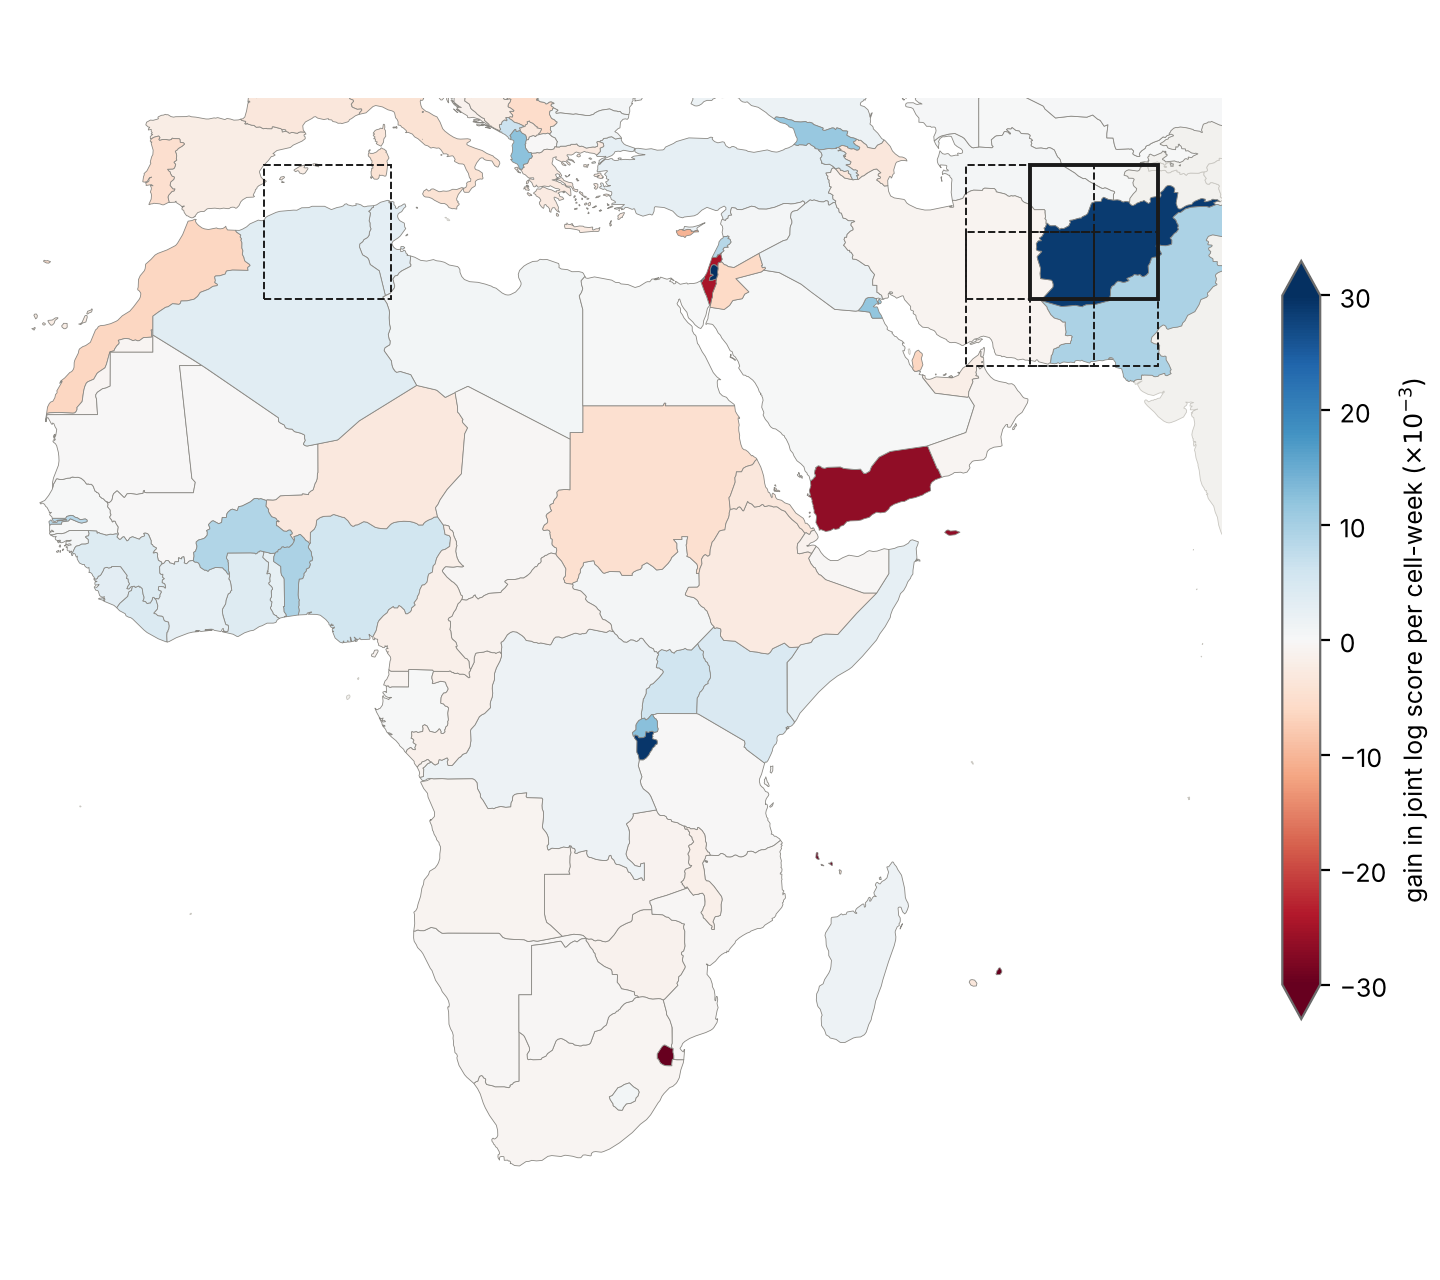
\includegraphics[width=0.85\textwidth]{figures/real_gain_map.png}
\caption{Gain in joint log score per cell-week of the joint model over the product of
the univariate static models, by country, on the 2023--2024 test period (blue: the
joint model predicts better). Boxes: the five $10^\circ \times 10^\circ$ windows with
the largest total gain on the 2022 validation year, selected without the test period;
solid: the first.}\label{fig:gain-map}
\end{figure}

\subsection{The boosting analysis before and after the repair}\label{sec:app-xgb}

Table~\ref{tab:app-xgb} reports three versions of the XGBoost analysis. The first,
\emph{as published}, applies the original procedure to the duplicated table: the
climate variables of the current week and their four-week means as features, positives
weighted by $(n_0/n_1)^{1/2}$, 5 million training rows sampled with replacement, and
the number of trees chosen by early stopping on the test years. The second,
\emph{deduplicated}, applies the same procedure unchanged to the repaired table. It
isolates the effect of the duplication and the leak. The third, \emph{corrected},
also changes the procedure. The number of trees is chosen by early stopping on 2022
after training on 2018--2021, and the model is then refitted on 2018--2022. It uses
no class weight. Its features use only information available before the week, so
the climate variables of the current week are dropped and only their four-week
means are kept. The 5 million training rows are sampled without replacement. The
weighted models are prior-corrected before scoring
(Section~\ref{sec:methods-hybrid}). We also fit the location-aware model of
Section~\ref{sec:methods-diagnostics}, which adds each cell's training event rate to
the corrected model. For the fit that chooses the number of trees, this rate uses
2018--2021 only; for the final fit it leaves out the row's own year.

On the duplicated table we recover the published performance, with AUC-PR 0.934
for conflict and 0.917 for unrest, against 0.93 and 0.91 reported. Split by cell,
nearly all of it comes from the cells that have copies in the original table (AUC-PR
0.966 and 0.968), and in the other cells AUC-PR is 0.498 and 0.528. The first two rows
of Table~\ref{tab:app-xgb} are on different test sets: the duplicated table has
14{,}425{,}130 test rows with conflict prevalence 2.98\%, the repaired table
4{,}787{,}224 rows with 1.62\%. AUC-PR depends on prevalence, so part of the difference
between them is not due to the model. Scored on one row per cell-week of the repaired
test set, the model fitted as published reaches AUC-PR 0.473 for conflict and 0.479
for unrest. The deduplicated and corrected rows are on identical test rows and can be
compared directly. Deduplication alone gives AUC-PR 0.546 for conflict and 0.555 for
unrest. The corrected model reaches 0.544 and 0.557, the persistence baseline 0.481
and 0.468, and the location-aware model 0.566 and 0.583. The scores are similar in
2023 and 2024. On onset rows, where the prevalence is 0.10\% for conflict and 0.14\%
for unrest, the corrected model reaches AUC-PR 0.0073 and 0.0097, and the
location-aware model 0.0111 and 0.0119.

Three conclusions follow. First, a flexible model of history and covariates improves
on persistence, but by less than the published scores suggest: the corrected model
improves on persistence by 0.06 in AUC-PR for conflict and 0.09 for unrest. This gain
cannot be attributed to the covariates alone. The persistence baseline uses only the
total count of the outcome, while the corrected model also uses the five event types
separately, including those of the other outcome, in a nonlinear way, together with
calendar indicators and country-year indicators whose joint values can identify a
country. Second, a cell intercept adds a
further 0.02 to 0.03, so part of what the covariates leave unexplained is persistent
and local. Third, on onset rows all models rank cell-weeks several times better than
chance, but their AUC-PR stays near 0.01. New events in places without recent events
are rarely anticipated.

\begin{table}
\caption{XGBoost on the 2023--2024 test period. As published: duplicated table,
original procedure (current-week features, class weight, early stopping on the test
years). Deduplicated: repaired table, original procedure. Corrected: repaired table,
features available before the week, no class weight, early stopping on 2022.
Corrected + cell event rate: the location-aware model. AUC-PR is also reported
separately for cells that have copies in the original table and for the others.
The persistence baseline ranks cell-weeks by the number of events in the previous four
weeks. The as-published rows are on a different test set from the other rows, with
a different prevalence.}\label{tab:app-xgb}
\centering\small
% Generated by paper/make_real_figures.py; do not edit by hand.
% Inputs (sha256 prefix):
%   results_real/xgb/metrics_corrected_Conflict.json  8fb209c4452d
%   results_real/xgb/metrics_corrected_Unrest.json  17d551c67437
%   results_real/xgb/metrics_corrected_te_Conflict.json  4342ad67c6f3
%   results_real/xgb/metrics_corrected_te_Unrest.json  c27a32300605
%   results_real/xgb/metrics_dedup_Conflict.json  046b10c52ba8
%   results_real/xgb/metrics_dedup_Unrest.json  5370f7674a41
%   results_real/xgb/metrics_original_Conflict.json  37a6e6e5b933
%   results_real/xgb/metrics_original_Unrest.json  9c4718f1c2d2
\begin{tabular}{@{}llrrrcccc@{}}
\toprule
Pipeline & Outcome & Test rows & Prevalence & Trees & AUC-PR & \multicolumn{2}{c}{AUC-PR by cell} & Persistence \\
\cmidrule(lr){7-8}
 & & & & & & dup.\ in original & other cells & AUC-PR \\
\midrule
As published & Conflict & 14.43M & 2.98\% & 1998 & 0.934 & 0.966 & 0.498 & 0.882 \\
As published & Unrest & 14.43M & 3.58\% & 1474 & 0.917 & 0.968 & 0.528 & 0.843 \\
\addlinespace
Original procedure, repaired table & Conflict & 4.79M & 1.62\% & 488 & 0.546 & 0.590 & 0.523 & 0.481 \\
Original procedure, repaired table & Unrest & 4.79M & 2.73\% & 646 & 0.555 & 0.543 & 0.558 & 0.468 \\
\addlinespace
Corrected & Conflict & 4.79M & 1.62\% & 637 & 0.544 & 0.588 & 0.521 & 0.481 \\
Corrected & Unrest & 4.79M & 2.73\% & 814 & 0.557 & 0.545 & 0.559 & 0.468 \\
\addlinespace
Corrected + cell event rate & Conflict & 4.79M & 1.62\% & 381 & 0.566 & 0.598 & 0.549 & 0.481 \\
Corrected + cell event rate & Unrest & 4.79M & 2.73\% & 135 & 0.583 & 0.567 & 0.586 & 0.468 \\
\bottomrule
\end{tabular}

\end{table}

\subsection{Residual spatial structure and the hybrid model}\label{sec:app-hybrid}

We fit the hybrid model~\eqref{eq:hybrid} to the AME region, that is Africa, the
Middle East and adjacent regions (longitude $20^\circ$W to $65^\circ$E, latitude
$36^\circ$S to $45^\circ$N; 13{,}719 cells in 93 countries, 4{,}976{,}634 cell-weeks of
which 1{,}426{,}776 are in the test period; Section~\ref{sec:data-acled}). It
combines the XGBoost offset cross-fitted by country, country effects, and either a
Mat\'ern field with sea barriers (Remark~\ref{rem:boundary}) or independent cell
effects. The offset is trained on the rows of this region only, whereas the corrected
XGBoost model of Section~\ref{sec:app-xgb} is trained on all locations worldwide.
The comparisons below are on identical test rows, but the training sets differ.

Table~\ref{tab:app-diag} reports the test-period residual diagnostics of
every model, and Figure~\ref{fig:app-variogram} the semivariograms of the
test-period residuals. The residuals of the corrected XGBoost model have Moran's $I$
of 0.42 for conflict and 0.15 for unrest (Section~\ref{sec:data-eda}). The
location-aware model reduces it to 0.29 for conflict but increases it to 0.25 for
unrest. The hybrid models do not reduce the overall test-period residual structure. For
conflict, Moran's $I$ is 0.45 with the field or with independent cell effects, about
the same as for the corrected model. For unrest it is 0.29, about twice the value of
the corrected model and above the 0.26 of the cross-fitted offset alone. For unrest,
latent effects estimated on the training years therefore increase the test-period
residual autocorrelation. One possible explanation is that cell effects estimated in
2018--2022 are carried into a period in which recorded unrest rose and its cell-level
pattern changed (Section~\ref{sec:data-acled}); the location-aware model shows a
similar increase. The hybrid models do reduce the residual correlation across borders,
from 0.21 to 0.14 for conflict and from 0.08 to $-0.02$ for unrest. Residual structure
in the test period is therefore not removed by latent effects estimated on the
training years. Section~\ref{sec:app-forecast} examines why. For the cross-fitted
offset, the across-border correlation is 0.25 for pairs of countries in the same fold
and 0.28 for pairs in different folds for conflict, and 0.14 and 0.09 for unrest.
The same-fold pairs are few (264 of 2{,}040).

Table~\ref{tab:app-field} gives the fitted hyperparameters. For
conflict, the field has range 263\,km and standard deviation 1.48. For unrest, the
range is 65\,km and the standard deviation 1.25. A range close to the size of a cell,
about 55~km at the equator, means that the field is not resolved by the grid
(Section~\ref{sec:methods-spde}). The field then behaves like independent cell
effects, and it should not be read as regional hotspots that cross borders. This is
the case for unrest. The field improves the log marginal likelihood over independent
cell effects by 1{,}254 for conflict but only by 95 for unrest, and the two give almost
the same test scores for unrest (Table~\ref{tab:app-forecast}). For unrest,
cell-level effects would largely track towns and cities, where protests are both more
frequent and more often reported. A fit to all locations worldwide (46{,}031 cells)
gives a range of 313\,km for conflict and 65\,km for unrest. The unrest results of the
AME region also depend on its composition. It includes Mediterranean Europe, where
unrest is dense and where several countries enter ACLED only in 2020
(Section~\ref{sec:data-acled}). The univariate analyses of this section use that
earlier region; the joint analyses of the main text exclude the countries of Europe,
and we have not repeated the univariate analyses on the restricted region.

Figure~\ref{fig:app-fitted} compares observed and predicted frequencies over the
test period. The hybrid model reproduces the regional pattern of both outcomes,
including the Sahel, eastern Congo, Somalia, Yemen and Syria--Iraq for conflict.
For both outcomes the hybrid model is close to the diagonal above a predicted
probability of about 1\% and overpredicts below it, where the observed frequency is
lower than predicted. The cross-fitted offset alone underpredicts in the same bins.

\begin{figure}
\centering
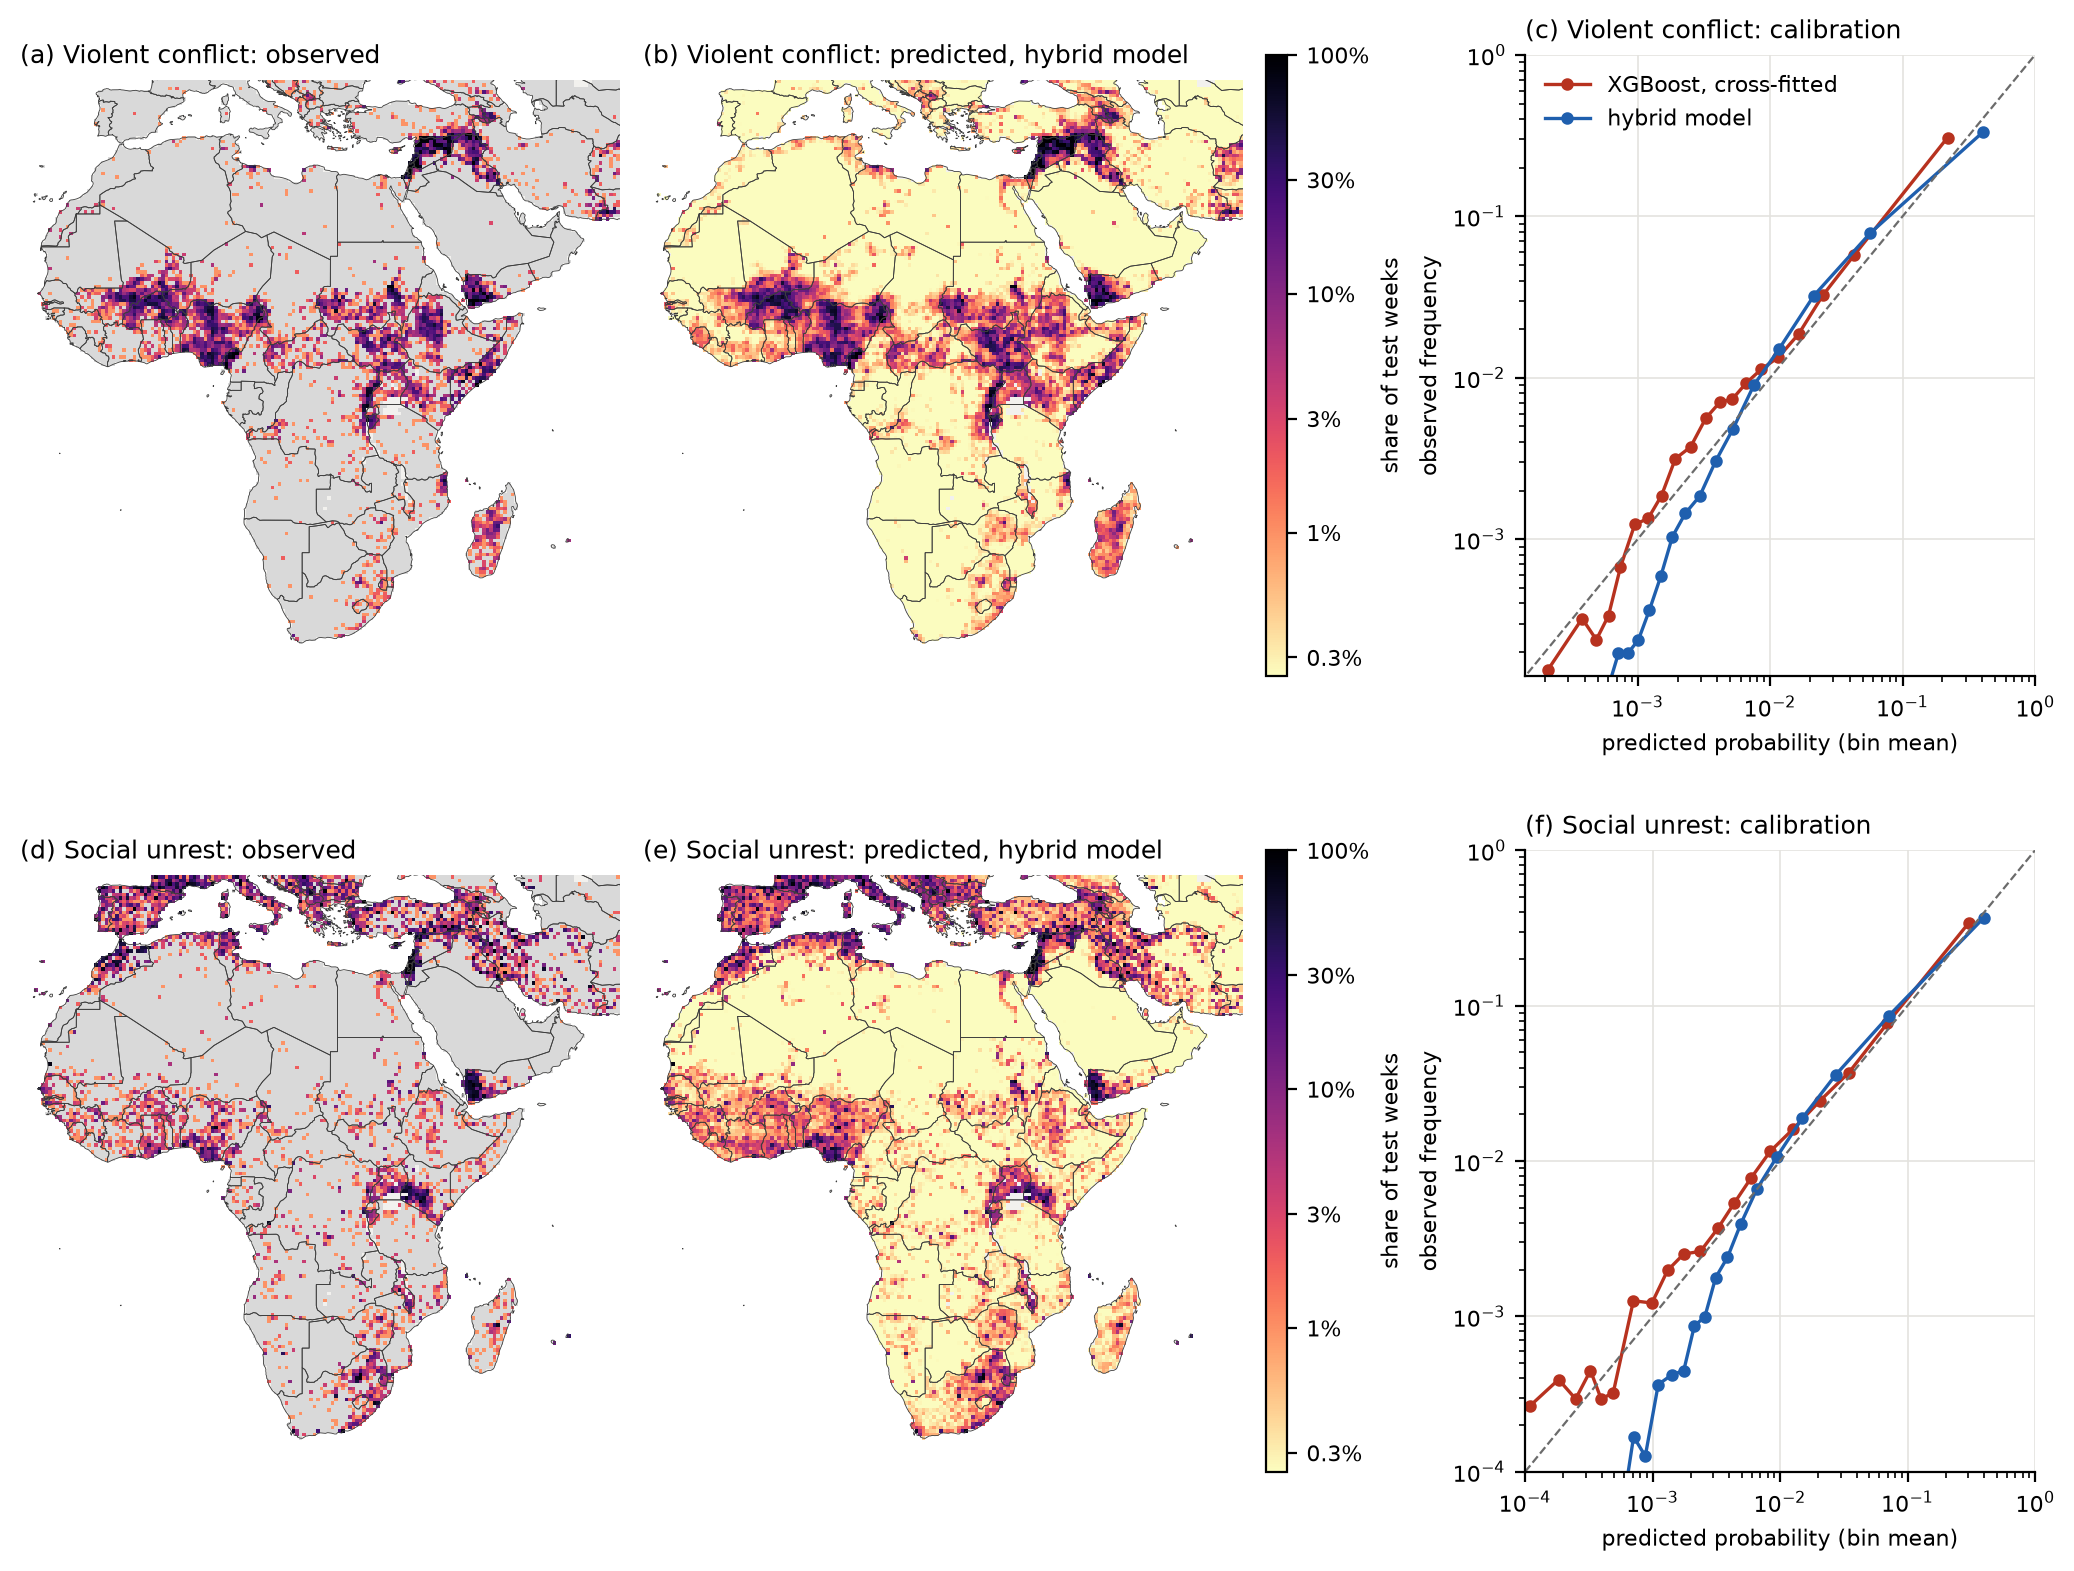
\includegraphics[width=\textwidth]{figures/real_fitted.png}
\caption{Observed and predicted event frequency in the test period 2023--2024,
AME region. (a, d) Share of test weeks with at least one event in each
cell; grey cells have no event week. (b, e) Mean predicted probability of the hybrid
model with country effects and the Mat\'ern field over the same weeks, on the same
colour scale. (c, f) Calibration: observed frequency against mean predicted probability
in 20 equal-count bins, for the hybrid model and the XGBoost offset cross-fitted by
country; the dashed line is perfect calibration.}\label{fig:app-fitted}
\end{figure}

The estimated fields are shown in Figure~\ref{fig:app-field}.
Table~\ref{tab:app-boxes} summarises the posterior of the field averaged
over eleven regions. The regions were chosen before the fit: eight known conflict
zones and three regions expected to be quiet. A posterior probability close to one
that the average over a known conflict zone is positive is therefore expected and is
not a finding in itself. The last two rows of the table give a summary that does not
depend on chosen regions: the share of cells whose posterior probability that
$w(s) > 0$ exceeds 0.95, and the share for which it is below 0.05. For conflict these
shares are 18.9\% and 3.0\%, and for unrest 11.6\% and 2.6\%. For conflict, the
averages over the three quiet regions, the western Congo basin, the interior of the
Arabian peninsula and southern Africa, are negative. For unrest, only the average
over eastern Congo is clearly positive, and none is clearly negative. Negative
values of $w$ mark low \emph{recorded} risk relative to the covariates, recent history
and country effects. In regions with restricted media access and few ACLED sources,
such as the interior of the Arabian peninsula, they may reflect reporting rather than
occurrence (Section~\ref{sec:data-acled}). Positive values in cells with towns or
administrative centres may in part reflect events of low spatial precision, which
ACLED places at such centroids. Because the offset is cross-fitted by country, errors
of the offset that are common to a country are absorbed by $u$, but errors that vary
within a country can be absorbed by $w$.

\begin{figure}
\centering
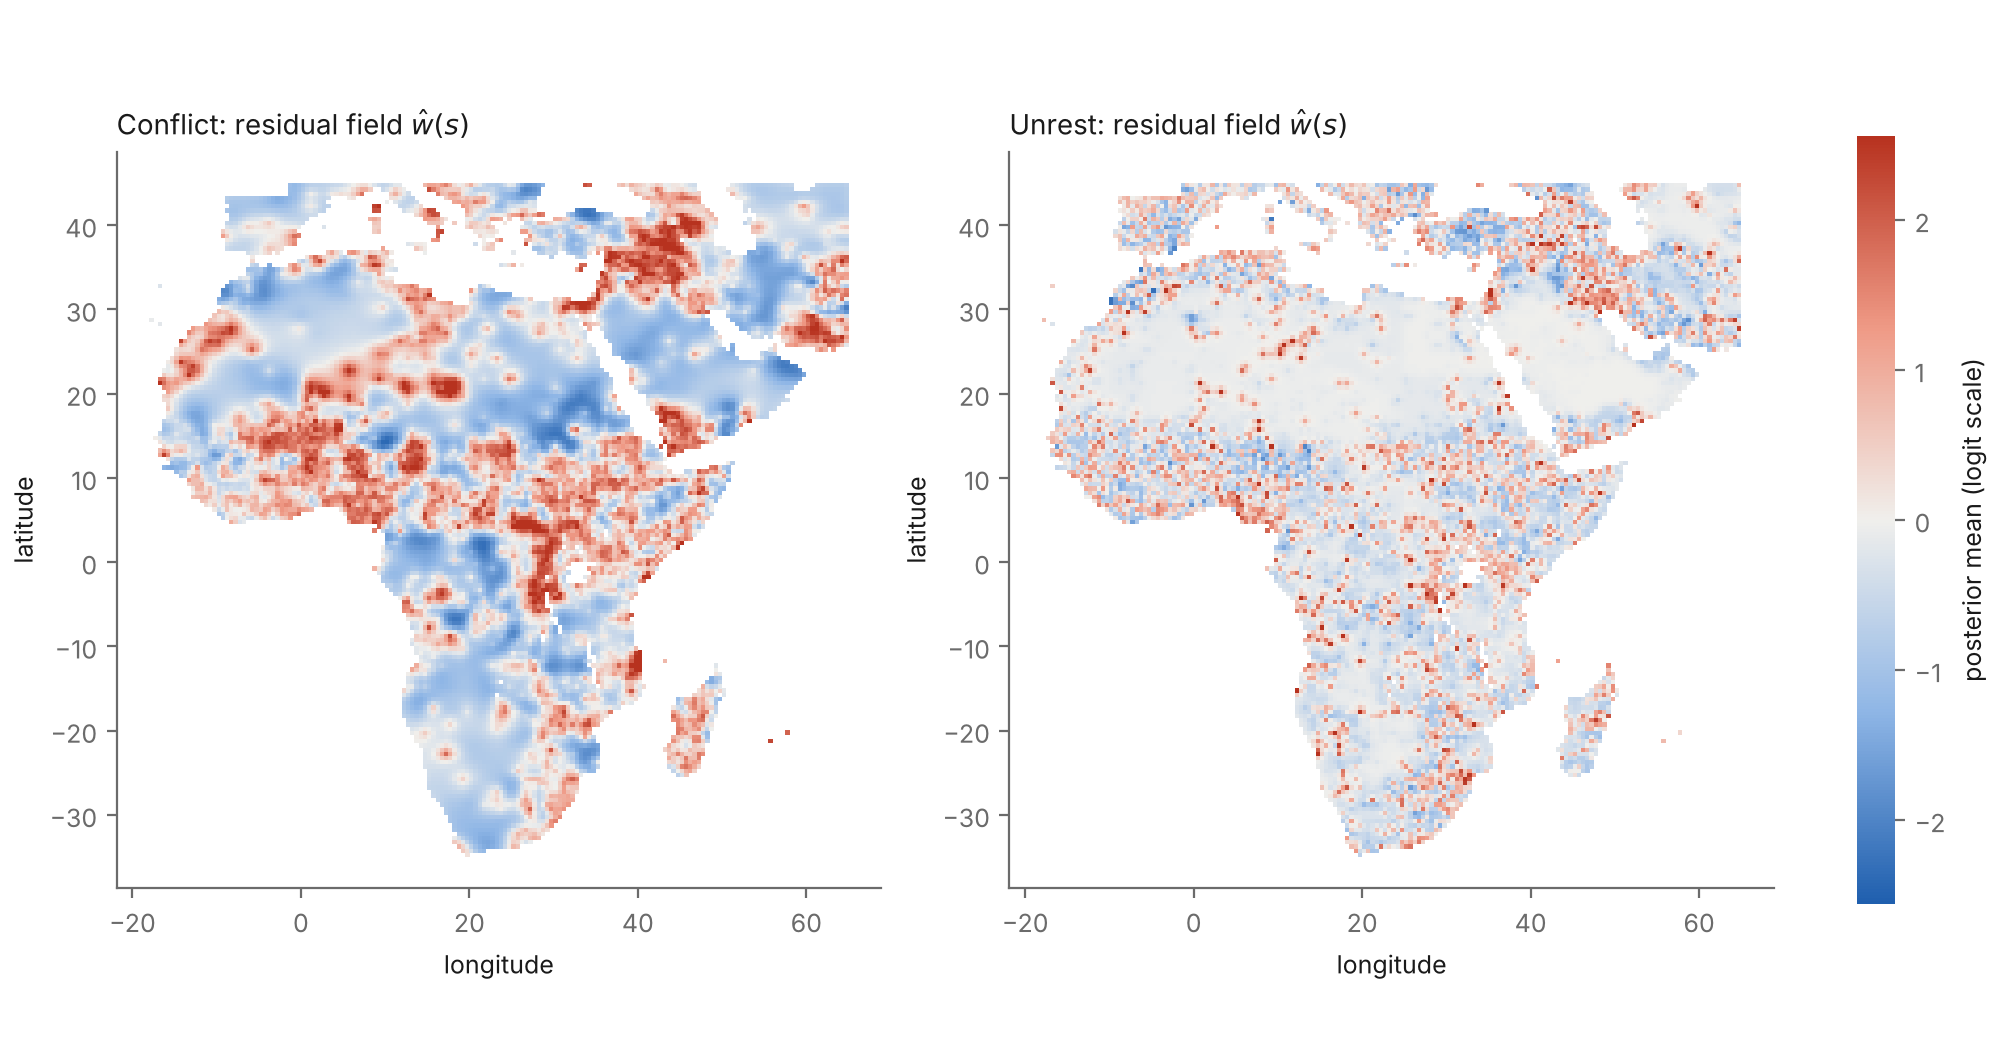
\includegraphics[width=\textwidth]{figures/real_field.png}
\caption{Posterior mean of the residual field $w(s)$ of the hybrid model for conflict
(left) and unrest (right), on the logit scale. Positive values mark higher recorded
risk than predicted by the covariates, recent event history and country effects.
Recorded risk mixes occurrence and reporting, and events of low spatial precision are
placed at town and administrative centroids (Section~\ref{sec:data-acled}).}\label{fig:app-field}
\end{figure}

\subsection{Forecasting}\label{sec:app-forecast}

Table~\ref{tab:app-forecast} compares out-of-sample scores on identical test rows of
the AME region. The reference is the corrected XGBoost model. Differences
in mean log score are given against it, with standard errors clustered by country
(standard errors clustered by cell are smaller). A gain of a hybrid model over the
cross-fitted offset alone is not evidence for the latent effects
(Section~\ref{sec:methods-hybrid}). The relevant comparisons are with the corrected
and location-aware models. The table has two parts. In the static part, every model
is fitted once on 2018--2022. In the updated part, the models are updated each
quarter of the test period with all data before the start of the quarter, as an
early-warning system would be run. The location-aware boosting model is updated by
recomputing the cell event rate. The hybrid models keep the hyperparameters fitted on
2018--2022 and recompute the latent effects. Table~\ref{tab:app-dynamic}
reports all dynamic experiments.

\paragraph{Static models.} With the field, the hybrid model improves on the corrected
XGBoost model in log score by 0.0021 (SE 0.0007) for unrest. For conflict the
difference, 0.0012 (SE 0.0009), is within about one standard error. The hybrid models
do not reach the location-aware model, which improves on the corrected model by
0.0035 (SE 0.0013) and 0.0032 (SE 0.0008). The Brier score, which
Table~\ref{tab:app-forecast} does not report, points the other way for conflict. The
hybrid model with the field has a Brier score higher than the corrected model by
0.0004 (SE 0.0002) for conflict, and lower by 0.0001 (SE 0.0002) for unrest. The
location-aware model lowers the Brier score by 0.0003 (SE 0.0002) and 0.0004
(SE 0.0002). The field and the independent cell effects
give almost the same scores: for conflict the field is better by 0.0002 in log score,
and for unrest by less than 0.0001. A hybrid model with a space-time field
($\Delta = 13$ weeks, forecast through its AR(1) dynamics) improves only slightly on
the static field, by 0.0004 for conflict and 0.0003 for unrest. In AUC-PR, the
corrected model reaches 0.515 for conflict and 0.532 for unrest, the hybrid model with
the field 0.519 and 0.540, the location-aware model 0.533 and 0.550, and persistence
0.446 and 0.451. On onset rows, where the prevalence is 0.15\% for conflict and 0.18\%
for unrest, AUC-PR is 0.008 to 0.011 for conflict and 0.010 to 0.014 for unrest for all
models except the cross-fitted offset alone, which reaches 0.006 and 0.009.

\paragraph{Updated models.} Quarterly updating improves every model that is updated;
the corrected XGBoost model and the cross-fitted offset are not updated. The updated
hybrid model with the space-time field improves on the corrected XGBoost model by
0.0035 (SE 0.0008) for conflict and 0.0034 (SE 0.0007) for unrest. It thus reaches the
score of the static location-aware model, and its AUC-PR is 0.539 and 0.554. It also
has the highest AUC-PR on onset rows, 0.0120 for conflict and 0.0142 for unrest.
Updating also improves the location-aware model, however, to 0.0050 (SE 0.0013) and
0.0044 (SE 0.0008) in log score, and AUC-PR 0.544 and 0.559. Of the gap in log score
between the static hybrid model with the field and the static location-aware model,
0.0023 for conflict and 0.0012 for unrest, a gap of 0.0015 and 0.0010 remains between
the best updated models of each kind. In the Brier score the updated space-time hybrid
model is better than the corrected model, by 0.0001 (SE 0.0001) for conflict and
0.0004 (SE 0.0002) for unrest, and the updated location-aware model by 0.0005
(SE 0.0002) and 0.0006 (SE 0.0002). The updated space-time hybrid model removes most
of the test-period residual structure: Moran's $I$ of its residuals is 0.12 for
conflict and 0.10 for unrest, against 0.32 and 0.26 for the updated location-aware
model.

We also refitted the hybrid models, including the boosting offset and the
hyperparameters, on 2018--2023 and scored 2024. These comparisons are on the 2024 rows
only. The refitted hybrid model with the field improves on the corrected model by
0.0022 for conflict and 0.0033 for unrest, against 0.0007 and 0.0017 without the
refit. The location-aware model, which is not refitted in this experiment, improves on
it by 0.0028 and 0.0023. A year of new data thus brings the hybrid model close to the
location-aware model for conflict and ahead of the static location-aware model for
unrest.

\paragraph{Where the residual structure lies.} To see why latent effects estimated on
the training years help little, we fitted the field and the independent cell effects
to the test period itself, with the same offset. This is an in-sample upper bound on
what a static latent term can absorb. For conflict, the test-period field has a range
of 374\,km, the field fits much better than independent cell effects (log marginal
likelihood higher by 1{,}045), and it removes the residual autocorrelation (Moran's $I$
from 0.54 to $-0.12$, against 0.35 with independent cell effects). Its correlation
with the field fitted on 2018--2022 is 0.79. For unrest, the test-period field has a
range of 66\,km, its advantage over independent cell effects is small (69 in log
marginal likelihood), and its correlation with the training field is 0.69. Conflict
residual risk is therefore smooth at a scale of a few hundred kilometres and partly
moves over time, which is why updating, and a space-time field, help. Unrest residual
risk is mainly cell-level, which is what a cell event rate captures directly. A
location-aware boosting model is a strong benchmark for both.

\begin{table}
\caption{Out-of-sample scores, AME region, 2023--2024, on identical
test rows. Static models are fitted once on 2018--2022; updated models are updated
each quarter with all data before the quarter (hybrid models: latent effects
recomputed with the hyperparameters fixed; location-aware model: cell event rate
recomputed). Differences in mean log score against the corrected XGBoost model, with
standard errors clustered by country. Lower is better for the log score. The hybrid
offset is trained on the AME region only; the corrected and
location-aware XGBoost models are trained on all locations. Onset rows: cells without
an event of the outcome in the previous 52 weeks. Further experiments in Table~\ref{tab:app-dynamic}.}\label{tab:app-forecast}
\centering\small
% Generated by paper/make_real_figures.py; do not edit by hand.
% Inputs (sha256 prefix):
%   results_real/compare/compare_conflict.json  f9cfaa08c2c7
%   results_real/compare/compare_conflict_st.json  41eadb9f67f6
%   results_real/compare/compare_conflict_update.json  e016ec0c6b38
%   results_real/compare/compare_unrest.json  b8e39ca9067c
%   results_real/compare/compare_unrest_st.json  8d037dd2f5c8
%   results_real/compare/compare_unrest_update.json  4c3deb048ccd
\resizebox{\textwidth}{!}{%
\begin{tabular}{@{}lcccccc@{}}
\toprule
Model & \multicolumn{3}{c}{Conflict} & \multicolumn{3}{c}{Unrest} \\
\cmidrule(lr){2-4}\cmidrule(lr){5-7}
 & AUC-PR & $\Delta$ log score & $\Delta$ Brier & AUC-PR & $\Delta$ log score & $\Delta$ Brier \\
 & & $\times 10^3$ (SE) & $\times 10^3$ (SE) & & $\times 10^3$ (SE) & $\times 10^3$ (SE) \\
\midrule
\multicolumn{7}{@{}l}{\emph{Fitted once on 2018--2022}} \\
\quad XGBoost, corrected (reference) & 0.515 & reference & reference & 0.532 & reference & reference \\
\quad XGBoost + cell event rate & 0.533 & $-3.50$ (1.27) & $-0.32$ (0.22) & 0.550 & $-3.22$ (0.78) & $-0.36$ (0.18) \\
\quad XGBoost, cross-fitted by country (offset) & 0.461 & $8.24$ (2.27) & $1.39$ (0.42) & 0.493 & $4.74$ (1.20) & $0.91$ (0.28) \\
\quad Offset + $u$ + iid cell effects & 0.519 & $-0.93$ (0.89) & $0.42$ (0.21) & 0.540 & $-2.04$ (0.67) & $-0.10$ (0.18) \\
\quad Offset + $u + w$ & 0.519 & $-1.17$ (0.94) & $0.44$ (0.23) & 0.540 & $-2.07$ (0.66) & $-0.10$ (0.18) \\
\quad Offset + $u$ + cell effects + $v$, 13-week steps & 0.519 & $-1.56$ (0.96) & $0.30$ (0.24) & 0.541 & $-2.33$ (0.79) & $-0.19$ (0.21) \\
\quad Offset + $u$ + cell effects + $v$, 26-week steps & 0.518 & $-1.52$ (0.95) & $0.34$ (0.25) & 0.540 & $-2.29$ (0.80) & $-0.17$ (0.22) \\
\addlinespace
\multicolumn{7}{@{}l}{\emph{Updated each quarter of the test period}} \\
\quad XGBoost + cell event rate & 0.544 & $-4.98$ (1.31) & $-0.54$ (0.23) & 0.559 & $-4.38$ (0.83) & $-0.59$ (0.17) \\
\quad Offset + $u$ + iid cell effects & 0.531 & $-2.30$ (0.76) & $0.12$ (0.14) & 0.550 & $-3.03$ (0.72) & $-0.35$ (0.18) \\
\quad Offset + $u + w$ & 0.531 & $-2.65$ (0.77) & $0.11$ (0.14) & 0.550 & $-3.06$ (0.72) & $-0.35$ (0.18) \\
\quad Offset + $u$ + cell effects + $v$, 13-week steps & 0.539 & $-3.52$ (0.81) & $-0.14$ (0.09) & 0.554 & $-3.39$ (0.71) & $-0.42$ (0.17) \\
\addlinespace
Persistence (past 4 weeks) & 0.446 & -- & -- & 0.451 & -- & -- \\
\bottomrule
\end{tabular}
}

\end{table}

\subsection{State dependence, climate and national indicators}\label{sec:app-glmm}

The parametric latent models of Section~\ref{sec:methods-model} are fitted to the AME
region (3{,}494{,}982 training rows, 13{,}719 cells). We compare
logistic regression without latent effects, a model with country effects, and models
with country effects, independent cell effects and a Mat\'ern field, with and without
a spatially varying coefficient for maximum temperature and with the spatial+
adjustment of Section~\ref{sec:methods-confounding}.

\paragraph{State dependence.} The coefficient $\delta$ of the own four-week history is
2.04 (SE 0.007) for conflict in logistic regression, 1.75 with country effects and
0.92 (SE 0.008) with country effects, cell effects and the field. For unrest it is
1.62, 1.47 and 0.78. The coefficient of the other outcome's history falls in the same
way, from 0.40 to 0.15 for unrest on conflict and from 0.22 to 0.13 for conflict on
unrest. In the central Sahel ($9^\circ$N to $20^\circ$N, $6^\circ$W to $16^\circ$E, a
box of $22^\circ$ by $11^\circ$; 968 cells, steps of 8 weeks), adding a space-time field
lowers $\hat\delta$ further: for conflict from 1.58 without latent effects to 0.65
with the static terms and 0.28 (SE 0.021) with the space-time field, whose range is
230\,km and AR(1) coefficient 0.93 per 8 weeks. For unrest the corresponding values
are 1.27, 0.42 and 0.17 (SE 0.060), with an AR(1) coefficient of 0.49 per 8 weeks,
about 0.915 per week. Much of the apparent state dependence is therefore absorbed by
latent risk that varies slowly in space and time. Three caveats apply. First, the
central Sahel models have no neighbour histories, so a space-time field at this scale
can also absorb diffusion of events between neighbouring cells. In West Africa,
adding the space-time field lowers the coefficient of conflict in neighbouring cells
from 0.129 (SE 0.007) to 0.051 (SE 0.008) (Table~\ref{tab:app-joint}). The fall in
$\hat\delta$ therefore cannot distinguish persistent latent risk from spatio-temporal
diffusion. Second, in S3 the empirical SD of $\hat\delta$ was 1.19 to 1.66 times its
mean SE whenever a space-time field was fitted, so the SEs above are too small,
by an amount that varies across settings. Third, the unrest dynamics are in the regime
of S3 ($\phi$ about 0.9 per week, $\Delta = 8$) in which $\hat\delta$ kept an upward
bias of about 0.10 under pure heterogeneity. The field $v$ is also defined on the
observed cells only, with reflecting edges, which departs from Remark~\ref{rem:boundary};
in the space-time hybrid models the same holds for the static part. $\hat\delta$ under
$v$ should be read with that caveat. As in S3 (Section~\ref{sec:sim-persistence}), we
read the remaining $\hat\delta$ as conditional dependence of recorded events
(Section~\ref{sec:methods-persistence}), not as contagion.

\paragraph{Climate.} All models condition on the event histories of the previous four
weeks and on the latent effects. The climate coefficients are therefore short-run
direct associations. Any effect of climate that acts through earlier events is
blocked, and we do not estimate total effects. In the model with the field, the
coefficients of the five standardised anomalies for conflict are 0.015 (SE 0.006) for
maximum temperature, $-0.007$ (SE 0.006) for minimum temperature, $-0.003$ (SE 0.005)
for precipitation, $-0.004$ (SE 0.004) for drought and 0.005 (SE 0.007) for
PM$_{2.5}$. For unrest they are 0.009 (SE 0.007), $-0.021$ (SE 0.006), $-0.017$
(SE 0.005), $-0.006$ (SE 0.004) and 0.033 (SE 0.007). The unrest coefficients of
minimum temperature and precipitation are thus 3 to 4 SE from zero and larger in
absolute value than that of maximum temperature. These SEs treat cell-weeks as
conditionally independent given the static latent effects, and residual space-time
dependence would make them too small, so we do not read the conflict coefficient of
maximum temperature, 2.5 SE from zero, as clear evidence. The PM$_{2.5}$ anomaly is
not interpretable. PM$_{2.5}$ is missing in 55.5\% of training rows and its
climatological standard deviation is undefined in 91{,}392 of the 164{,}628
cell-months, so the floor is about $10^{-9}$ and standardised anomalies can be
extreme (Section~\ref{sec:data-cov}). Of the five, we examine the maximum-temperature
anomaly in more detail. The biome-specific slopes of the model with a spatially varying coefficient lie
between $-0.16$ and $0.08$ for conflict and between $-0.09$ and $0.06$ for unrest, and
none is more than two standard errors from zero. The spatially varying part has
standard deviation 0.076 for conflict and 0.072 for unrest, so variation within biomes
is negligible, and the model does not improve the marginal likelihood or the test
scores over the model without it. Conditional on recent event history and the latent
effects, the short-run direct association of maximum-temperature anomalies with the
weekly probability of recorded events is therefore small in the AME region, and we find
no evidence that it differs between or within biomes. This statement does not extend
to the other anomalies, nor to total effects of climate.

\paragraph{National indicators.} Without latent effects, several between-country
coefficients are large and estimated with standard errors below 0.02, for example
$-0.56$ (SE 0.008) for the EPI on conflict and 0.12 (SE 0.005) for the liberal
democracy index on unrest. With country effects their standard errors grow by an order
of magnitude, and with the field they change further: $-0.22$ (SE 0.12) for the EPI on
conflict and 0.21 (SE 0.14) for the liberal democracy index on unrest. They are also
unstable under spatial+: for the EPI on conflict $-0.23$, $-0.22$ and $-0.07$ with
$m = 10$, 20 and $m^* = 138$, and for the liberal democracy index on unrest 0.17, 0.20
and $-0.02$ with $m = 10$, 20 and $m^* = 176$. In the light of S2
(Section~\ref{sec:sim-confounding}), the between-country coefficients cannot be
separated from spatially smooth unmeasured risk, and we do not interpret them.

The within-country coefficients are identified from changes over time within a
country. Across the models with the field (with the field, with the spatially varying
coefficient, and spatial+), they barely change, for example 0.014 to 0.016 for the EPI
on conflict and 0.030 for the liberal democracy index on unrest. They are not all
small. In the model with the field, the within coefficients on conflict are 0.095
(SE 0.007) for log GDP per capita, $-0.082$ (SE 0.011) for greenhouse gas emissions and
0.049 (SE 0.010) for the ecological footprint, several times the
maximum-temperature coefficient. Their standard errors, however, treat cell-weeks as
conditionally independent, whereas the within variation comes from about 93 countries
over five training years. Like the between coefficients, they rest on few independent
contrasts, and their model-based standard errors are too small by an unknown amount.
We therefore do not interpret them either. Access to electricity needs a further
caveat. Unlike the other national indicators, it is not re-attached per country and
year in the repaired table (Section~\ref{sec:data-acled}), so in cells that had copies
it can carry the value of a neighbouring country. Its within component then mixes
change over time with differences across borders. This may explain why its within
coefficient on conflict is $-0.106$ (SE 0.005) without latent effects but $-0.027$
(SE 0.023) with the field, and on unrest 0.008 (SE 0.006) without latent effects but
0.072 (SE 0.024) with the field. We do not interpret the electricity coefficients.

\paragraph{Missingness.} Two missingness indicators were dropped because they are
constant in the training rows (EPI and liberal democracy index), and the material and
ecological footprint indicators were merged with that of greenhouse gas emissions. The
remaining indicators are not interpretable as effects. They vary mostly between
countries, so they are confounded with the country effects and the field, and their
signs change across specifications. For a missing GDP the coefficient on conflict is
0.31 (SE 0.022) without latent effects, $-0.08$ (SE 0.061) with country effects and
$-0.26$ (SE 0.056) with the field. For a missing IPC analysis the coefficient on unrest
is 0.06 (SE 0.020), 0.20 (SE 0.023) and $-0.18$ (SE 0.030) in the same three models.
The other indicators have large standard errors, and we do not interpret any of them.


\section{Additional tables}\label{supp:tables}

\begin{table}
\caption{Latent blocks of the latent Gaussian model of Section~3.1 of the main paper, their precision matrices and
hyperparameters.}\label{tab:blocks}
\centering\small
\begin{tabular}{@{}llll@{}}
\toprule
Block & Dimension & Precision & Hyperparameters \\
\midrule
fixed effects $\bbeta, \delta, \bm{\alpha}$ & $p$ & $10^{-4} \bm{I}$ & -- \\
country effects $\bu$ & $n_c$ & $\sigma_u^{-2} \bm{I}$ & $\sigma_u$ \\
spatial field $\bw$ & $n$ & $\bQ_s(\rho_w, \sigma_w)$, SPDE precision & $\rho_w, \sigma_w$ \\
cell effects $\bm{e}$ & $n$ & $\sigma_e^{-2} \bm{I}$ & $\sigma_e$ \\
space-time field $\bv$ & $n\,T_v$ & $\bQ_{\mathrm{AR}}(\phi) \otimes \bQ_s(\rho_v, \sigma_v)$ & $\rho_v, \sigma_v, \phi$ \\
\bottomrule
\end{tabular}
\end{table}

\begin{table}
\caption{Boundary treatments on a $60 \times 30$ lattice of $0.5^\circ$ cells with
a sea strait of 2, 4 or 6 cells (about 110, 220, 330\,km): marginal variance of a
coastal and of an inland land cell (nominal 1) and correlation between the two
coastal cells facing each other across the strait, from 4{,}000 exact draws with
$\rho = 400$\,km. ``Land only'' removes the strait from the lattice; ``sea = land''
keeps it as ordinary cells without data. The strait lies inside a closed rectangle.
This is not the geometry of the application, which has an open coast, a buffer of sea
cells and a reflecting outer edge, and the fitted ranges there are both above and
below 400\,km, so the table shows the behaviour of the barrier only
qualitatively.}\label{tab:barrier}
\centering\small
\begin{tabular}{@{}llrrrrr@{}}
\toprule
Strait & & Land only & Sea = land & $f=0.1$ & $f=0.2$ & $f=0.5$ \\
\midrule
2 cells & var.\ coast & 1.98 & 1.07 & 1.80 & 1.67 & 1.29 \\
 & var.\ inland & 1.10 & 1.06 & 1.09 & 1.11 & 1.09 \\
 & corr.\ across & -0.01 & 0.49 & -0.03 & 0.01 & 0.16 \\
\addlinespace
4 cells & var.\ coast & 2.00 & 1.08 & 1.77 & 1.69 & 1.29 \\
 & var.\ inland & 1.06 & 1.05 & 1.09 & 1.09 & 1.09 \\
 & corr.\ across & 0.00 & 0.28 & 0.01 & 0.01 & 0.04 \\
\addlinespace
6 cells & var.\ coast & 2.02 & 1.04 & 1.76 & 1.66 & 1.26 \\
 & var.\ inland & 1.06 & 1.05 & 1.08 & 1.07 & 1.07 \\
 & corr.\ across & -0.02 & 0.14 & 0.01 & 0.01 & 0.01 \\
\bottomrule
\end{tabular}

\end{table}

\begin{table}
\caption{S2: full results for the escalation effect $\kappa$ of recent unrest on
conflict, by scenario and estimator, over 20 replicates per scenario. Mean
$\hat\kappa$, its empirical SD across replicates and the mean of the estimated SEs;
coverage of the nominal 95\% intervals for $\kappa$ with its Monte Carlo SE;
proportion of replicates whose interval excludes zero; mean estimate of the own-lag
coefficient $d_c$ (truth 0.3); mean and SD of the estimated loading $\lambda$ of the
shared space-time field (truth 0.8, joint model only); and mean log score, AUC-PR and
onset AUC-PR of the conflict forecasts over the 26 test weeks. Onset rows are those of
cells without a conflict event in the previous 52 weeks. The last two scenarios add
unrest-only episodes (AR(1) with coefficient 0.95, Mat\'ern innovations of range
200\,km, marginal SD 0.6), which the joint model with one shared field must absorb
into that field.}\label{tab:s5}
\centering\small
\resizebox{\textwidth}{!}{\begin{tabular}{@{}lcccccccccc@{}}
\toprule
Estimator & Mean $\hat\kappa$ & Emp.\ SD & Mean SE & Coverage & Reject & Mean & Mean $\hat\lambda$ & Log & AUC-PR & Onset \\
 & & & & (MC SE) & $\kappa = 0$ & $\hat d_c$ & (SD) & score & & AUC-PR \\
\midrule
\multicolumn{11}{@{}l}{\emph{No escalation, $\kappa = 0$}} \\
\quad Logistic regression & 0.695 & 0.193 & 0.129 & 0.05 (0.05) & 0.95 & 1.54 & -- & 0.1372 & 0.063 & 0.022 \\
\quad Static field $w_c$ & 0.426 & 0.161 & 0.135 & 0.15 (0.08) & 0.85 & 0.82 & -- & 0.1335 & 0.090 & 0.037 \\
\quad Static field $w_c$ + space-time field & 0.269 & 0.158 & 0.140 & 0.45 (0.11) & 0.55 & 0.38 & -- & 0.1341 & 0.090 & 0.034 \\
\quad Joint model, shared space-time field & 0.042 & 0.166 & 0.138 & 0.90 (0.07) & 0.10 & 0.38 & 0.83 (0.14) & 0.1343 & 0.088 & 0.033 \\
\addlinespace
\multicolumn{11}{@{}l}{\emph{Escalation, $\kappa = 0.4$}} \\
\quad Logistic regression & 1.026 & 0.163 & 0.116 & 0.00 (0.00) & 1.00 & 1.52 & -- & 0.1430 & 0.077 & 0.025 \\
\quad Static field $w_c$ & 0.794 & 0.128 & 0.122 & 0.10 (0.07) & 1.00 & 0.80 & -- & 0.1392 & 0.105 & 0.044 \\
\quad Static field $w_c$ + space-time field & 0.659 & 0.108 & 0.127 & 0.50 (0.11) & 1.00 & 0.37 & -- & 0.1399 & 0.105 & 0.045 \\
\quad Joint model, shared space-time field & 0.434 & 0.111 & 0.126 & 0.95 (0.05) & 0.95 & 0.36 & 0.83 (0.15) & 0.1401 & 0.103 & 0.042 \\
\bottomrule
\end{tabular}
}
\end{table}

\begin{table}
\caption{Joint model of conflict and unrest, by region (Section~5 of the
main paper): all hyperparameters and lag coefficients (posterior mean, with SE in
parentheses) of the two univariate conflict models and of the joint model, fitted on
2018--2022. Subscripts C and U denote conflict and unrest. In the univariate model with
$u + e + w + v$, the space-time field $v$ belongs to conflict alone; in the joint model
it is shared, with loading $\lambda$ for unrest. Histories are $\log(1 + \text{events
in the previous four weeks})$; neighbour histories are means over the rook neighbours,
standardised on the training rows. The log marginal likelihood of the joint model
includes the unrest data and is not comparable with those of the univariate models.
Test scores are for 2023--2024 in the same region. The field $v$ is defined on the
observed $1^\circ$ cells only, with reflecting edges, which departs from the boundary
rule of Remark~1 of the main paper. SEs are plug-in values; in S1 and S2 such SEs are
too small when a space-time field is fitted (ratio of empirical SD to mean SE up to
1.66 in S1 and 1.20 in S2 without escalation), so intervals from these models are
likely too narrow. With a single shared space-time field, unrest-only episodes are
absorbed into $v$, which can bias $\kappa$ towards zero; in S2 they inflated
$\hat\lambda$ instead. The extended model has an additional unrest-specific space-time field $v_{\mathrm{U}}$. Test scores here use the probit approximation to $E\{\operatorname{expit}(\eta)\}$; the model comparisons in the text use common Monte Carlo draws.}\label{tab:app-joint-full}
\centering\small
% Generated by paper/make_real_figures.py; do not edit by hand.
% Inputs (sha256 prefix):
%   results_real/bivariate/west_sahel/summary_biv.json  ea44c0cdfc8a
%   results_real/bivariate/west_sahel/summary_biv2.json  33869b8129ae
%   results_real/bivariate/africa_me/summary_biv.json  6ec2bb2906f6
%   results_real/bivariate/africa_me/summary_biv2.json  cc7e24f4d08e
\begin{tabular}{@{}lcccc@{}}
\toprule
Quantity & Conflict only & Conflict only & Joint & Joint \\
 & $u + e + w$ & $u + e + w + v$ & shared $v$ & shared $v$ + $v_{\mathrm{U}}$ \\
\midrule
\multicolumn{5}{@{}l}{\emph{West Africa and Sahel}} \\
\multicolumn{5}{@{}l}{\quad 2{,}505 cells, 22 countries, 906{,}810 rows per outcome} \\
\multicolumn{5}{@{}l}{\quad $v$ on 641 observed $1^\circ$ cells (reflecting edges), 28 steps of 13 weeks} \\
\multicolumn{5}{@{}l}{Hyperparameters} \\
\quad $\sigma_{u,\mathrm{C}}$ & 0.69 & 0.67 & 0.69 & 0.67 \\
\quad $\sigma_{e,\mathrm{C}}$ & 0.65 & 0.64 & 0.66 & 0.65 \\
\quad $\rho_{w,\mathrm{C}}$ (km) & 514 & 508 & 453 & 467 \\
\quad $\sigma_{w,\mathrm{C}}$ & 1.70 & 1.74 & 1.39 & 1.44 \\
\quad $\sigma_{u,\mathrm{U}}$ & -- & -- & 0.53 & 0.51 \\
\quad $\sigma_{e,\mathrm{U}}$ & -- & -- & 1.34 & 1.36 \\
\quad $\rho_{w,\mathrm{U}}$ (km) & -- & -- & 369 & 497 \\
\quad $\sigma_{w,\mathrm{U}}$ & -- & -- & 0.21 & 0.34 \\
\quad $\rho_v$ (km) & -- & 423 & 499 & 445 \\
\quad $\sigma_v$ & -- & 0.69 & 1.01 & 0.99 \\
\quad $\phi$ (per step) & -- & 0.905 & 0.952 & 0.957 \\
\quad $\lambda$ & -- & -- & 0.868 & 0.580 \\
\quad $\rho_{v,\mathrm{U}}$ (km) & -- & -- & -- & 787 \\
\quad $\sigma_{v,\mathrm{U}}$ & -- & -- & -- & 0.49 \\
\quad $\phi_{\mathrm{U}}$ (per step) & -- & -- & -- & 0.687 \\
\multicolumn{5}{@{}l}{Conflict equation} \\
\quad $\delta_{\mathrm{C}}$: own history & $0.575$ (0.016) & $0.444$ (0.017) & $0.459$ (0.017) & $0.448$ (0.017) \\
\quad $\kappa$: unrest history & $0.138$ (0.031) & $0.131$ (0.032) & $0.044$ (0.032) & $0.095$ (0.032) \\
\quad $\delta^{\mathrm{nb}}_{\mathrm{C}}$: neighbours' conflict & $0.129$ (0.007) & $0.051$ (0.008) & $0.061$ (0.008) & $0.054$ (0.008) \\
\quad $\kappa^{\mathrm{nb}}$: neighbours' unrest & $0.005$ (0.008) & $0.003$ (0.008) & $-0.020$ (0.008) & $-0.005$ (0.008) \\
\multicolumn{5}{@{}l}{Unrest equation} \\
\quad $\delta_{\mathrm{U}}$: own history & -- & -- & $0.351$ (0.029) & $0.269$ (0.029) \\
\quad $\kappa_{\mathrm{U}}$: conflict history & -- & -- & $0.066$ (0.031) & $0.111$ (0.031) \\
\quad $\delta^{\mathrm{nb}}_{\mathrm{U}}$: neighbours' unrest & -- & -- & $0.017$ (0.009) & $-0.004$ (0.009) \\
\quad $\kappa^{\mathrm{nb}}_{\mathrm{U}}$: neighbours' conflict & -- & -- & $-0.042$ (0.013) & $-0.008$ (0.014) \\
\multicolumn{5}{@{}l}{Fit} \\
\quad Log marginal likelihood & $-49530.1$ & $-49080.6$ & $-76591.8$ & $-76461.0$ \\
\quad Fit time (h) & 0.1 & 0.7 & 4.5 & 8.2 \\
\quad Test AUC-PR, conflict & 0.470 & 0.471 & 0.466 & 0.470 \\
\quad Test log score, conflict & 0.1020 & 0.1026 & 0.1031 & 0.1029 \\
\quad Test AUC-PR, unrest & -- & -- & 0.289 & 0.283 \\
\quad Test log score, unrest & -- & -- & 0.0490 & 0.0496 \\
\addlinespace
\multicolumn{5}{@{}l}{\emph{AME region}} \\
\multicolumn{5}{@{}l}{\quad 13{,}719 cells, 93 countries, 4{,}921{,}758 rows per outcome} \\
\multicolumn{5}{@{}l}{\quad $v$ on 3{,}637 observed $1^\circ$ cells (reflecting edges), 14 steps of 26 weeks} \\
\multicolumn{5}{@{}l}{Hyperparameters} \\
\quad $\sigma_{u,\mathrm{C}}$ & 0.50 & 0.50 & 0.53 & 0.52 \\
\quad $\sigma_{e,\mathrm{C}}$ & 0.96 & 0.97 & 0.99 & 0.99 \\
\quad $\rho_{w,\mathrm{C}}$ (km) & 562 & 583 & 632 & 598 \\
\quad $\sigma_{w,\mathrm{C}}$ & 1.63 & 1.60 & 1.20 & 1.21 \\
\quad $\sigma_{u,\mathrm{U}}$ & -- & -- & 0.90 & 0.93 \\
\quad $\sigma_{e,\mathrm{U}}$ & -- & -- & 1.31 & 1.32 \\
\quad $\rho_{w,\mathrm{U}}$ (km) & -- & -- & 439 & 417 \\
\quad $\sigma_{w,\mathrm{U}}$ & -- & -- & 0.35 & 0.48 \\
\quad $\rho_v$ (km) & -- & 480 & 486 & 472 \\
\quad $\sigma_v$ & -- & 0.87 & 1.25 & 1.26 \\
\quad $\phi$ (per step) & -- & 0.873 & 0.946 & 0.948 \\
\quad $\lambda$ & -- & -- & 0.668 & 0.440 \\
\quad $\rho_{v,\mathrm{U}}$ (km) & -- & -- & -- & 697 \\
\quad $\sigma_{v,\mathrm{U}}$ & -- & -- & -- & 0.43 \\
\quad $\phi_{\mathrm{U}}$ (per step) & -- & -- & -- & 0.696 \\
\multicolumn{5}{@{}l}{Conflict equation} \\
\quad $\delta_{\mathrm{C}}$: own history & $0.794$ (0.008) & $0.603$ (0.009) & $0.626$ (0.009) & $0.608$ (0.009) \\
\quad $\kappa$: unrest history & $0.150$ (0.014) & $0.133$ (0.015) & $0.057$ (0.015) & $0.105$ (0.015) \\
\quad $\delta^{\mathrm{nb}}_{\mathrm{C}}$: neighbours' conflict & $0.175$ (0.004) & $0.070$ (0.004) & $0.083$ (0.004) & $0.073$ (0.004) \\
\quad $\kappa^{\mathrm{nb}}$: neighbours' unrest & $-0.004$ (0.006) & $-0.007$ (0.006) & $-0.035$ (0.006) & $-0.015$ (0.006) \\
\multicolumn{5}{@{}l}{Unrest equation} \\
\quad $\delta_{\mathrm{U}}$: own history & -- & -- & $0.585$ (0.009) & $0.542$ (0.009) \\
\quad $\kappa_{\mathrm{U}}$: conflict history & -- & -- & $0.025$ (0.014) & $0.074$ (0.014) \\
\quad $\delta^{\mathrm{nb}}_{\mathrm{U}}$: neighbours' unrest & -- & -- & $0.071$ (0.004) & $0.057$ (0.004) \\
\quad $\kappa^{\mathrm{nb}}_{\mathrm{U}}$: neighbours' conflict & -- & -- & $-0.042$ (0.006) & $-0.008$ (0.007) \\
\multicolumn{5}{@{}l}{Fit} \\
\quad Log marginal likelihood & $-173069.3$ & $-170579.1$ & $-354668.9$ & $-353977.4$ \\
\quad Fit time (h) & 0.1 & 0.7 & 6.4 & 4.7 \\
\quad Test AUC-PR, conflict & 0.524 & 0.522 & 0.526 & 0.525 \\
\quad Test log score, conflict & 0.0593 & 0.0600 & 0.0595 & 0.0597 \\
\quad Test AUC-PR, unrest & -- & -- & 0.541 & 0.534 \\
\quad Test log score, unrest & -- & -- & 0.0640 & 0.0646 \\
\bottomrule
\end{tabular}

\end{table}

\begin{table}
\caption{S1: estimation of the state-dependence parameter $\delta$ for all five truths
and all step lengths of the space-time field $v$ (20 replicates per truth). The two
truths with slow $v$ have an AR(1) coefficient of 0.97 per week instead of 0.9. SD/SE
is the ratio of the empirical SD of $\hat\delta$ to the mean estimated SE; values
above 1 mean that the plug-in intervals are too narrow. Time is the mean fit time per
replicate.}\label{tab:s3-full}
\centering\small
\begin{tabular}{@{}lcccccc@{}}
\toprule
Estimator & Mean $\hat\delta$ & Emp.\ SD & Mean SE & SD/SE & Coverage & Time (s) \\
\midrule
\multicolumn{7}{@{}l}{\emph{State dependence ($\delta = 1$)}} \\
\quad Lags only & 1.263 & 0.107 & 0.136 & 0.78 & 0.60 & 0.1 \\
\quad Lags + $w$ & 1.032 & 0.131 & 0.139 & 0.94 & 0.90 & 0.9 \\
\quad Lags + $w$ + $v$ (8-week steps) & 0.981 & 0.128 & 0.140 & 0.92 & 0.95 & 27.3 \\
\quad Lags + $w$ + $v$ (4-week steps) & 0.990 & 0.135 & 0.140 & 0.96 & 0.95 & 101.5 \\
\quad Lags + $w$ + $v$ (weekly steps) & 0.997 & 0.143 & 0.140 & 1.02 & 0.95 & 449.6 \\
\addlinespace
\multicolumn{7}{@{}l}{\emph{Heterogeneity ($\delta = 0$)}} \\
\quad Lags only & 1.614 & 0.386 & 0.099 & 3.88 & 0.00 & 0.1 \\
\quad Lags + $w$ & 0.464 & 0.093 & 0.111 & 0.84 & 0.00 & 1.0 \\
\quad Lags + $w$ + $v$ (8-week steps) & 0.097 & 0.140 & 0.117 & 1.19 & 0.80 & 26.4 \\
\quad Lags + $w$ + $v$ (4-week steps) & 0.045 & 0.152 & 0.119 & 1.28 & 0.90 & 95.1 \\
\quad Lags + $w$ + $v$ (weekly steps) & 0.011 & 0.162 & 0.120 & 1.35 & 0.90 & 474.2 \\
\addlinespace
\multicolumn{7}{@{}l}{\emph{Mixed ($\delta = 0.5$)}} \\
\quad Lags only & 1.659 & 0.351 & 0.106 & 3.32 & 0.00 & 0.1 \\
\quad Lags + $w$ & 0.782 & 0.111 & 0.115 & 0.96 & 0.25 & 1.0 \\
\quad Lags + $w$ + $v$ (8-week steps) & 0.567 & 0.144 & 0.119 & 1.21 & 0.85 & 24.6 \\
\quad Lags + $w$ + $v$ (4-week steps) & 0.545 & 0.152 & 0.120 & 1.27 & 0.85 & 90.0 \\
\quad Lags + $w$ + $v$ (weekly steps) & 0.535 & 0.172 & 0.120 & 1.43 & 0.80 & 349.7 \\
\addlinespace
\multicolumn{7}{@{}l}{\emph{Heterogeneity, slow $v$ ($\delta = 0$, $\phi = 0.97$ per week)}} \\
\quad Lags only & 1.649 & 0.418 & 0.100 & 4.18 & 0.00 & 0.1 \\
\quad Lags + $w$ & 0.384 & 0.115 & 0.113 & 1.01 & 0.05 & 1.0 \\
\quad Lags + $w$ + $v$ (8-week steps) & 0.037 & 0.160 & 0.119 & 1.35 & 0.90 & 25.7 \\
\quad Lags + $w$ + $v$ (4-week steps) & 0.006 & 0.170 & 0.119 & 1.42 & 0.95 & 91.8 \\
\quad Lags + $w$ + $v$ (weekly steps) & -0.013 & 0.165 & 0.120 & 1.37 & 0.90 & 464.9 \\
\addlinespace
\multicolumn{7}{@{}l}{\emph{Mixed, slow $v$ ($\delta = 0.5$, $\phi = 0.97$ per week)}} \\
\quad Lags only & 1.650 & 0.367 & 0.107 & 3.42 & 0.00 & 0.1 \\
\quad Lags + $w$ & 0.711 & 0.144 & 0.118 & 1.22 & 0.55 & 1.0 \\
\quad Lags + $w$ + $v$ (8-week steps) & 0.503 & 0.194 & 0.121 & 1.60 & 0.85 & 22.9 \\
\quad Lags + $w$ + $v$ (4-week steps) & 0.491 & 0.198 & 0.122 & 1.63 & 0.85 & 84.0 \\
\quad Lags + $w$ + $v$ (weekly steps) & 0.479 & 0.203 & 0.122 & 1.66 & 0.85 & 468.4 \\
\bottomrule
\end{tabular}

\end{table}

\IfFileExists{spr-ims-nameyear.bst}{\bibliographystyle{spr-ims-nameyear}}{\bibliographystyle{plainnat}}
\bibliography{refs}

\end{document}
